\documentclass[
  reprint,
  amsmath,
  amssymb,
  aps,
  pra,
  nofootinbib,
  superscriptaddress,
  floatfix
]{revtex4-2}

\usepackage[T1]{fontenc}
\usepackage{lmodern}
\usepackage{graphicx}
\graphicspath{{../../}{}}
\usepackage{capt-of} % \captionof for non-floating figures (used with widetext)
\usepackage{booktabs}
\usepackage{bm}
\usepackage{mathtools}
\usepackage{amsthm}
\usepackage{xcolor}
\usepackage{hyperref}

\newcommand{\placeholder}[1]{\textcolor{red!70!black}{\ifmmode\left[#1\right]\else\textsf{[#1]}\fi}}
\newcommand{\tentative}[1]{\textcolor{red!70!black}{#1}}
\newcommand{\structlabel}[1]{\noindent\mbox{\tentative{#1.}}~}
\newcommand{\Oset}{\mathcal{O}}
\newcommand{\Gset}{\mathcal{G}}
\newcommand{\Rset}{\mathcal{R}}
\newcommand{\Sset}{\mathcal{S}}
\newcommand{\Hcal}{\mathcal{H}}
\newcommand{\Bcal}{\mathcal{B}}
\newcommand{\Ocal}{\mathcal{O}}
\newcommand{\Ucal}{\mathcal{U}}
\newcommand{\Jcal}{\mathcal{J}}
\newcommand{\Pcal}{\mathcal{P}}
\newcommand{\Dcal}{\mathcal{D}}
\newcommand{\Mcal}{\mathcal{M}}
\newcommand{\Wcal}{\mathcal{W}}
\newcommand{\dd}{\mathrm{d}}
\newcommand{\ii}{\mathrm{i}}
\newcommand{\ee}{\mathrm{e}}
\newcommand{\TR}{\mathrm{TR}}
\newcommand{\ex}{\mathrm{ex}}
\newcommand{\ctrl}{\mathrm{ctrl}}
\newcommand{\stat}{\mathrm{stat}}
\newcommand{\dyn}{\mathrm{dyn}}
\newcommand{\drv}{\mathrm{drv}}
\newcommand{\obs}{\mathrm{obs}}
\newcommand{\stay}{\mathrm{stay}}
\newcommand{\app}{\mathrm{append}}
\newcommand{\ablate}{\mathrm{ablate}}
\newcommand{\Var}{\operatorname{Var}}
\newcommand{\Tr}{\operatorname{Tr}}
\newcommand{\Top}{\operatorname{Top}}
\newcommand{\argminp}{\mathop{\mathrm{arg\,min}}}
\newcommand{\argmaxp}{\mathop{\mathrm{arg\,max}}}
\newcommand{\proj}{\mathrm{proj}}
\newcommand{\diag}{\mathrm{diag}}
\newcommand{\CVaR}{\operatorname{CVaR}}
\newcommand{\softmax}{\operatorname{softmax}}
\newcommand{\hh}{\mathrm{HH}}
\newcommand{\phmax}{n_{\mathrm{ph,max}}}
\newcommand{\twq}{\mathrm{2Q}}
\newcommand{\eps}{\varepsilon}
\newcommand{\ket}[1]{|#1\rangle}
\newcommand{\bra}[1]{\langle #1|}
\newcommand{\braket}[2]{\langle #1|#2\rangle}
\newcommand{\expval}[1]{\langle #1\rangle}
\newcommand{\inlinetablecaption}[2]{%
  \refstepcounter{table}\label{#1}%
  \noindent\textsc{Table~\thetable.} #2\par\vspace{0.6ex}%
}
\newenvironment{schurlemma}[1][]
{\par\medskip\noindent\textbf{Lemma}\if\relax\detokenize{#1}\relax\else\ (#1)\fi.\space\itshape}
{\par\medskip}
\newenvironment{schurassumption}[1][]
{\par\medskip\noindent\textbf{Assumption}\if\relax\detokenize{#1}\relax\else\ (#1)\fi.\space}
{\par\medskip}
\newenvironment{schurtheorem}[1][]
{\par\medskip\noindent\textbf{Theorem}\if\relax\detokenize{#1}\relax\else\ (#1)\fi.\space\itshape}
{\par\medskip}
\newenvironment{schurremark}[1][]
{\par\medskip\noindent\textbf{Remark}\if\relax\detokenize{#1}\relax\else\ (#1)\fi.\space}
{\par\medskip}


\begin{document}

\title{Geometry- and Cost-Aware ADAPT Ansatz Construction for Mixed Fermion--Boson Hamiltonians}

\author{Jake Strobel}
\author{Jacopo Simoni}
\author{Gabrielle Riva}
\author{Yuan Ping}
\affiliation{University of Wisconsin--Madison}

\date{\today}



\begin{abstract}
Mixed fermion--boson Hamiltonians combine electronic correlation with truncated bosonic motion, producing compact few-site benchmarks whose informative observables are already difficult for noisy quantum processors because two-qubit depth, measurement burden, and variational refit cost grow rapidly.  We present SNAKE, a geometry- and cost-aware ADAPT procedure for ground-state ansatz construction.  Candidate generators are promoted to candidate--position records and scored through lower-confidence Fubini--Study trust-region gain, hardware and measurement cost penalties, tangent novelty, Schur-refit reranking, batching, beam continuation, and rollback-safe generator ablation.  SNAKE reaches the target accuracy across fermionic, bosonic, and mixed fermion--boson benchmarks, with its largest separation on mixed systems: at fixed energy accuracy, it reduces compiled two-qubit count by \(\placeholder{XX}\), two-qubit depth by \(\placeholder{YY}\), total circuit depth by \(\placeholder{GG}\), and shot count by \(\placeholder{KK}\) relative to the best non-SNAKE ADAPT competitor.
\end{abstract}

\maketitle



\section{Introduction}

\structlabel{Problem, Hamiltonian, importance of solving it}
Mixed fermion--boson Hamiltonians describe weakly to strongly coupled many-body problems in which electronic correlation, lattice motion, and electron--phonon dressing jointly determine the relevant eigenstates and observables \cite{Hubbard1963,Holstein1959a,Holstein1959b}.  Important examples include Hubbard, Hubbard--Holstein, spin-boson, molecular electronic, and vibronic instances.  A standard objective in condensed-matter, molecular, and quantum-simulation applications is approximating low-energy states of the Hilbert space in order to determine site-resolved densities/occupations, doublon correlations, phonon dressing, and mode-resolved bosonic occupation.  Ground-state preparation can further provide the basis for variational real-time dynamics and subspace-based excited-state spectra \cite{LiBenjamin2017VQS,Yuan2019VQS,McClean2017QSE}.

Classical solvers are effective for small system sizes, though increasing orbital number, lattice size, and bosonic cutoff rapidly enlarge the truncated Hilbert space.  Exact diagonalization scales cubically with Hilbert dimension \cite{Weisse2008}; sparse eigensolvers scale with Hamiltonian sparsity and the requested low-energy subspace \cite{Schollwock2011}; tensor-network cost can grow with entanglement-controlled bond dimension and bosonic local dimension \cite{Schollwock2011}; and quantum Monte Carlo can encounter sign- or phase-problem scaling \cite{Troyer2005}.  Qubit encodings can reduce the register component of this scaling pressure by representing an \(N\)-level local bosonic cutoff with \(O(\log N)\) qubits \cite{Sawaya2020,Li2023}.  On current quantum processors, the bottleneck then shifts to efficient ansatz--circuit compilation because errors compound with entangling depth, routing, and repeated measurements.

We consider Hamiltonians with the generic decomposition \cite{Dutta2024BosonicChemistry,Peng2025BosonHamiltonians}
\begin{align}
H&=H_f+H_b+H_{fb},
\nonumber\\
H_f&=\sum_{pq}h_{pq}c_p^\dagger c_q
+\frac12\sum_{pqrs}V_{pqrs}c_p^\dagger c_q^\dagger c_s c_r,
\nonumber\\
H_b&=\sum_{\mu}\omega_\mu b_\mu^\dagger b_\mu+H_b^{\rm nl},
\nonumber\\
H_{fb}&=\sum_{\mu}X_\mu^{(b)}F_\mu^{(f)}
+\sum_{\mu}P_\mu^{(b)}G_\mu^{(f)},
\label{eq:general_fb_terms_static}
\end{align}
where $X_\mu^{(b)}=b_\mu^\dagger+b_\mu$ and $P_\mu^{(b)}=\ii(b_\mu^\dagger-b_\mu)$, while $F_\mu^{(f)}$ and $G_\mu^{(f)}$ denote fermionic density/orbital-transition operators coupled to the bosonic displacement and momentum quadratures.  Hubbard, Hubbard--Holstein, boson-only, spin-boson, molecular electronic, and vibronic instances are treated as limiting cases, with specific benchmark forms given in Appendix~\ref{app:hamiltonian_families}.  For qubit representation, we use Jordan--Wigner fermionic encodings together with binary bosonic encodings and blocked fermionic/bosonic registers, fixed within each benchmark instance.

\structlabel{Current solution strategies}
NISQ ground-state algorithms usually minimize a Rayleigh--Ritz objective on a parameterized circuit \cite{Peruzzo2014,McClean2016,Kandala2017},
\begin{equation}
E(\theta)=
\bra{\psi_{\rm ref}}U^\dagger(\theta)HU(\theta)\ket{\psi_{\rm ref}},
\label{eq:rayleigh_static}
\end{equation}
where \(\ket{\psi_{\mathrm{ref}}}\) is typically a Hartree--Fock determinant \(\ket{\mathrm{HF}}\); for mixed systems with phonon truncation \(n_{\mathrm{cut}}\), we set \(\ket{\psi_{\mathrm{ref}}}=\ket{\mathrm{HF}}\otimes\ket{0_1\,0_2\,\cdots\,0_{n_{\mathrm{cut}}}}\).  Here \(U(\theta)\) denotes the ansatz unitary, with \(\theta\) its variational parameter vector. The ansatz structure can be chosen in advance, as in fixed-structure VQE \cite{Peruzzo2014,McClean2016,Kandala2017}, or grown iteratively, as in ADAPT-VQE \cite{Grimsley2019,Tang2021,Yordanov2021}. In the ADAPT case, a generator \(A^\star\) is selected from a predefined pool \(\mathcal G\) by maximizing the local energy-gradient objective,
\begin{equation}
A_k^\star=\arg\max_{A\in\mathcal G}
\left|
\left.
\partial_{\theta_A}E\!\left(e^{\theta_A A}U_k(\theta)\ket{\psi_{\mathrm{ref}}}\right)
\right|_{\theta_A=0}
\right|,
\end{equation}
and appending it to the ansatz,
\begin{equation}
U_{k+1}(\theta,\theta_A)=e^{\theta_A A_k^\star}U_k(\theta).
\end{equation}
In either case, the parameterization update rule is
\begin{equation}
\label{eq:theta_opt}
\theta^\star=\arg\min_\theta E(\theta).
\end{equation}
Recent variants improve circuit compactness by batching compatible generators (TETRIS-ADAPT) \cite{Anastasiou2024}, using operator sequencing with coupled-exchange strategies (CEO-ADAPT) \cite{Ramoa2025}, and promoting novel tangent directional growth (Overlap-ADAPT) \cite{Feniou2023}. Although traditional ADAPT uses first-order gradient information to expand the circuit, second-order information improves convergence \cite{Grimsley2023ADAPT} and allows the warm-start of parameters across iterations to cut optimizer overhead \cite{Ramoa2025HessianRecycling}. Concurrent with this work, Geo-ADAPT-VQE further improved convergence by replacing the \(\theta\)-space Euclidean metric with a state-space Fubini--Study metric within Eq.~(5) operator-selection score, and enabled generator insertion instead of append-only \cite{Sohail2026GeoADAPT}. In a similiar vein, Prune ADAPT tracks plaussibly archaic generators to ablate based off amplitude and iteration history \cite{Vaquero2025PrunedADAPT}.

\structlabel{Problem with current solutions}
Standard ADAPT, Qubit-ADAPT, and qubit-excitation ADAPT select operators from first-order energy gradients \cite{Grimsley2019,Tang2021,Yordanov2021} and remain susceptible to gradient plateaus and local-minimum traps \cite{Feniou2023,Grimsley2023ADAPT}. Although TETRIS-ADAPT improves circuit compactness by adding multiple high-gradient, qubit-disjoint operators in the same ADAPT iteration, it still inherits the same first-order plateau issue \cite{Anastasiou2024}. A common correction for first-order stagnation is a second-order derivative signal \cite{Ramoa2025HessianRecycling}. Because these methods score parameter-space derivatives, coordinate sensitivity can be mistaken for physical state-space displacement \cite{ProvostVallee1980,Stokes2020QNG}. Geo-ADAPT corrects this parameter-space defect by scoring operators with the Fubini--Study metric rather than a Euclidean treatment \cite{Sohail2026GeoADAPT}; however, this introduces an inverse pool-metric dependency, which can become rank-deficient or ill-conditioned in overcomplete or heterogeneous operator pools where distinct generators induce null, duplicate, or nearly redundant tangent directions. The integration of Fubini--Study/QIM scoring with second-order curvature, batching, and pruning remains an open additional complexity.

Two oversights remain across these variants: (1) an iteration-independent shot budget can overpay early and underpay late stage due to the iteration-dependent decrease in candidate signal-to-noise ratio \cite{Ikhtiarudin2025ShotEfficient}, and (2) absent a cost penalty, a candidate operator with a marginal gradient advantage can score higher despite having arbitrarily greater circuit-burden.

\structlabel{Solution strategy}
To avoid parameter-coordinate sensitivity and unreduced inverse pool-metric dependence, SNAKE evaluates operator-position records with a regularized Fubini--Study metric \cite{Sohail2026GeoADAPT}. SNAKE incorporates a second-order Taylor model into the energy-gradient objective of Eq. (3), but constrains the maximization to a geometric trust region \cite{Nocedal2006TrustRegion}. SNAKE allows a local-reparameterization window to avoid full-ansatz reparameterization after each admission; this window is the coordinate set used by the Schur reduction. The reduced Schur model ranks candidates by residual trust-region gain after accounting for coupling between existing ansatz tangent directions and candidate tangents under mutual reparameterization through a regularized Hessian treatment.

Then, degenerately scored candidates can be admitted jointly via TETRIS-ADAPT \cite{Anastasiou2024}, conditional on tangent nonredundancy. Under degenerate batch candidacy, SNAKE borrows Lowerre-style beam search to branch candidate circuits in parallel, with branch pruning upon dominance or budget pressure \cite{Lowerre1976Beam}.

To reduce persistent circuit cost, SNAKE enables a nested Schur ladder that analytically qualifies local recoverability under generator ablation \cite{Vaquero2025PrunedADAPT}. SNAKE further down-regulates circuit burden by an inter-pool variance weighting within the gradient-descent objective, penalizing candidate scoring by proxied two-qubit, circuit-depth, and shot burden \cite{Verteletskyi2020CliqueCover,Yen2020CompatibleMeasurements,Ikhtiarudin2025ShotEfficient}.

SNAKE uses tripartite scoring phases with intermittent quadripartite shortlisting based on Pauli support and commutation status. This shortlisting limits shot overhead by restricting expensive metric, curvature, and Schur evaluations to candidates that survive algebraically partitioned prior-phase scoring.

The generator-position record set is iteration-dependent. As the ansatz matures, local-reparameterization windows contract, shortlist pressure increases, expensive phases retire, and shot counts rise as candidate signal-to-noise decreases.

Finally, SNAKE is evaluated on fermionic, bosonic, and mixed fermion--boson Hamiltonians. Fixed-structure VQE has been applied to bosonic qumode/model Hamiltonians and to bosonic or supersymmetric high-energy matrix models \cite{Dutta2026QumodeVQE,Rinaldi2022MatrixModels,Dao2025SU2MatrixVQE}; however, to our knowledge, no ADAPT-VQE method has been demonstrated on condensed-matter bosonic or mixed fermion--boson Hamiltonians such as the bosonic-chain and Hubbard--Holstein families considered here. We compare against leading fixed-structure VQE and ADAPT competitors under shared Hamiltonian parameterization, encoding, and operator pools.

Appendix~\ref{app:schur_convergence} shows that, in the idealized single-record limit, Schur reduction removes the diagonal-dominance assumption required by Geo-ADAPT's selected-coordinate descent step. The proof derives a one-record descent certificate directly from the reduced Schur-refitted curve. The resulting stationarity and conditional global-convergence statements then follow by the standard summable-perturbation and QGI template.

The name SNAKE, State--Novel ADAPT Kost Evaluator, reflects the joint state-tangent-directed novelty \(\mathcal N\) and cost \(K\) objectives; pictorially, generator-sequence tail truncation with biased head growth iteratively traverses state space.



\section{SNAKE ADAPT ansatz-construction procedure}

\begin{center}
\centering
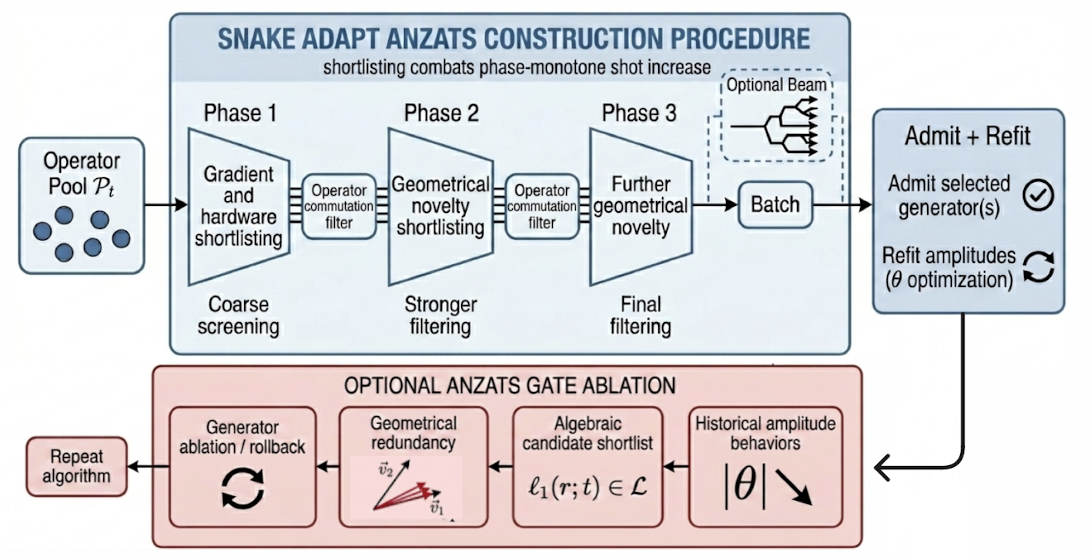
\includegraphics[width=\columnwidth]{figures/static_adapt_selector_flow_attached.png}
\captionof{figure}{SNAKE static ADAPT generator-selection flow. The broad generator pool is reduced through staged gradient--cost scoring, commutation filtering, algebraic identity shortlisting, final batch-compatible record selection, optional beam branching, and post-admission generator-ablation feedback.}
\label{fig:static_adapt_selector_flow}
\end{center}

\label{sec:static_method}

\subsection{Phase-zero and three-phase generator-position ranking}

SNAKE implements generator selection as a cheap Phase-0 pilot followed by a three-phase restriction of a candidate record set, beginning from all admissible generator--position pairs and ending with records eligible for insertion, batching, or beam branching, while a separate ablation check acts on stale entries of the existing ansatz.

Define generator set $\Gset$, and position set $\Pcal$,
\begin{equation}
\begin{aligned}
\Gset&=\{A_1,\ldots,A_m,\ldots,A_{|\Gset|}\},\\
\Pcal
&=
\left\{
p\in W(\theta;t)
\;\middle|\;
W(\theta;t)\subseteq\{1,\ldots,|U(\theta)|+1\}
\right\},
\end{aligned}
\label{eq:generator_position_sets}
\end{equation}
where $W(\theta;t)$ is a rolling window of admissible insertion positions of the existing ordered ansatz $U(\theta)$.  Define the mapping
\begin{equation}
\Phi:(\Gset,\Pcal)\longrightarrow
\mathcal R
=
\{r=(m,p)\mid A_m\in\Gset,\;p\in\Pcal\},
\label{eq:record_mapping}
\end{equation}
so $\mathcal R$ is the full candidate position-generator record set. For the staged recursion, set $\mathcal R_{-1}:=\mathcal R$, let $k\in\{0,1,2,3\}$ index the pilot or scoring phase, and let $\ell\in\mathcal L$ index the four-lane partition induced by the Cartesian product of qubit-support overlap and windowed operator-commutation status. Each stage maps $\mathcal R_{k-1}$ to $\mathcal R_k$ by lane-wise score thresholding
\begin{equation}
\mathcal R_k
:=
\bigcup_{\ell\in\mathcal L}
\left\{
r\in\mathcal R_{k-1}
\;\middle|\;
S_{k,\ell}(r)\ge\tau_{k,\ell}
\right\}.
\label{eq:phase_restriction_map}
\end{equation}
The phase score is
\begin{equation}
S_{k,\ell}(r)
=
\frac{\Delta E_k(r)\mathcal N_k(r)}{K_k(r)}.
\label{eq:master_phase_score}
\end{equation}
Here $\Delta E_k(r)$ is the phase-$k$ state-gradient gain, $\mathcal N_k(r)\in[0,1]$ is the geometric novelty factor ($\mathcal N_k(r)=1$ for $k\in\{0,1\}$), and $K_k(r)$ is the hardware-cost penalty ($K_k(r)\ge1$). The lane set satisfies $|\mathcal L|=4$, and $\tau_{k,\ell}$ is a phase- and lane-dependent threshold determined by candidate-record inter-competition. This provides the Eq.~(4)-analogous ansatz update rule,
\begin{equation}
U_{t+1}(\theta_{t+1})
=
U_t(\theta_t)
\oplus
\bigcup_{r_i\in\mathcal B\subseteq\mathcal R_3}r_i
\ominus
\bigcup_{d_j\in\mathcal D\subseteq U_t(\theta_t)}d_j .
\label{eq:snake_ansatz_update}
\end{equation}
Here $\mathcal B$ is the batch-admissible set of retained Phase-III records, and $\mathcal D$ is the ablation-admissible set of existing ansatz entries.

\subsubsection{Hardware cost penalty}

The phase-$k$ hardware-cost penalty is built from raw burden proxies for two-qubit count, layout-aware depth, new parameters, and shot demand. Consider the compiled generator, $A_m=\sum_{\nu}a_{m\nu}P_{m\nu}$ where $P_{m\nu}$ is a tensor-product of Pauli matrices and identities, $\sigma \in \{I,X,Y,Z\}$. Define the Pauli-support, $S_{m\nu}:=\operatorname{supp}(P_{m\nu})=\{q:(P_{m\nu})_q\ne I\}$. Then, for a Pauli exponential compiled by a CNOT ladder, the total 2q gate count is given by,
\begin{equation}
\widehat C_{\twq}(r)=\sum_{\nu}2\,[|S_{m\nu}|-1]_+,
\label{eq:pauli_2count_proxy}
\end{equation}
whereas the layout-aware two-qubit depth is given by,
\begin{equation}
\widehat C_d(r)=\sum_{\nu}2\,\operatorname{span}_{G}
\bigl(S_{m\nu}\bigr),
\label{eq:pauli_2depth_proxy}
\end{equation}
where $G=(V,E)$ is the qubit-hardware QPU graph and $\operatorname{span}_{G}(S)$ is the number of edges in the shortest connected subgraph containing $S$, and is zero for $|S|\le1$. The new-parameter feature is the increase in parameter-vector length from adding the candidate scalar coordinate $\vartheta_r$,
\begin{equation}
\widehat C_\theta(r)
=
|\theta\oplus\vartheta_r|-|\theta|.
\label{eq:parameter_cost_proxy}
\end{equation}
For measurement burden, the gradient observable associated with Eq.~(\ref{eq:resolved_gradient}) is partitioned into qubit-wise commuting groups $O_{r,b}=\sum_{\nu\in B_{r,b}}c_{r,b\nu}P_{r,b\nu}$. If $\mathcal B_r$ denotes this grouped Pauli partition, the per-candidate shot proxy scales as,
\begin{equation}
\widehat C_{\rm shot}(r)=
\frac{1}{\sigma_\star^2}
\left(
\sum_{b\in\mathcal B_r}
\sqrt{\sum_{\nu\in B_{r,b}}|c_{r,b\nu}|^2}
\right)^2,
\label{eq:shot_cost_proxy}
\end{equation}
with $\sigma_\star$ the target standard error for the candidate-gradient estimate \cite{Ikhtiarudin2025ShotEfficient}.

For a nonnegative raw feature $\widehat C_x$, the normalized excess cost is
\begin{equation}
\bar C_x(r;k):=
\operatorname{asinh}
\left(
\frac{[\widehat C_x(r)-m_x(k)]_+}{s_x(k)}
\right),
\label{eq:cost_robust_excess}
\end{equation}
where $m_x(k)$ and $s_x(k)$ are the median and robust positive scale over the live phase-$k$ record family. Measurement-grouping work supports treating Pauli burden as part of the adaptive algorithmic cost \cite{Verteletskyi2020CliqueCover,Yen2020CompatibleMeasurements}.

The final phase-$k$ hardware-cost penalty is one plus the weighted sum of these robust-normalized excess features,
\begin{equation}
\begin{aligned}
K_k(r)
={}&
1+\lambda_{\twq}\bar C_{\twq}(r;k)
+\lambda_d \bar C_d(r;k)\\
&+\lambda_\theta \bar C_\theta(r;k)
+\lambda_{\rm shot}\bar C_{\rm shot}(r;k),
\end{aligned}
\label{eq:hardware_cost_sum}
\end{equation}
where each barred feature is Eq.~(\ref{eq:cost_robust_excess}) applied to its corresponding raw proxy, so $K_k(r)\ge1$.

\subsubsection{Gradient-resolution envelope}

For a candidate record $r$, SNAKE estimates the finite-resolution floor
\begin{equation}
\eta_r(t)=z_\alpha\sigma_r(t)+b_r(t),
\label{eq:gradient_resolution_floor}
\end{equation}
where $\sigma_r(t)$ is the standard error of the gradient estimate, $z_\alpha$ fixes the confidence level, and $b_r(t)$ is a backend-resolution estimate computed from hardware metrics such as compiled circuit burden, gate/readout error, coherence exposure, mitigation residuals, and calibration drift; details are given in Appendix~\ref{app:gradient_resolution_floor}. The raw ADAPT gradient and resolved gradient are
\begin{equation}
\begin{aligned}
g_r(t)
&=
\left.
\partial_\alpha
\langle\psi_t|
e^{i\alpha\widetilde A_r}
H
e^{-i\alpha\widetilde A_r}
|\psi_t\rangle
\right|_{\alpha=0}\\
&=
i\langle\psi_t|[\widetilde A_r,H]|\psi_t\rangle,\\
\widetilde g_r(t)
&=|g_r(t)|-\eta_r(t),
\end{aligned}
\label{eq:resolved_gradient}
\end{equation}
lower bounded by zero in implementation. The Phase-I--III gain models below use this resolved gradient whenever a gradient magnitude enters a trust-region gain.

\subsubsection{Phase 0}

Phase 0 is the $k=0$ specialization of Eq.~(\ref{eq:master_phase_score}). It uses the upper-confidence first-order gradient envelope, scaled by a small pilot amplitude $\alpha_0>0$, as a pilot gain,
\begin{equation}
G_0^{\rm upper}(r;t)=|g_r(t)|+\eta_r(t),
\qquad
\Delta E_0(r;t)=\alpha_0 G_0^{\rm upper}(r;t),
\label{eq:phase0_gain}
\end{equation}
so that
\begin{equation}
S_{0,\ell}(r)=\frac{\Delta E_0(r;t)}{K_0(r)}.
\label{eq:phase0_score}
\end{equation}
This removes records whose optimistic pilot energy signal is insufficient before Fubini--Study or higher-order geometric scoring.

\subsubsection{Algebraic shortlisting}

After Phase 0 assigns each candidate--position record a pilot gradient and cost score, SNAKE preserves algebraically distinct survivors before the more expensive tangent-geometry evaluation. For $r$, let $\mathcal C_1(r;t)$ denote the generators in its local candidate context, including local pool neighbors and inherited-window generators. For each $A_n\in\mathcal C_1(r;t)$, the selector checks support overlap and commutation,
\begin{equation}
\operatorname{supp}(A_m)\cap\operatorname{supp}(A_n),
\qquad
[A_m,A_n].
\label{eq:algebraic_shortlist_checks}
\end{equation}
For Pauli-expanded generators, let $N_{\rm ac}(m,n)$ be the number of sites in the shared support where $P_q^{(m)}$ and $P_q^{(n)}$ anticommute. The commutation test is
\begin{equation}
[A_m,A_n]=0
\quad\Longleftrightarrow\quad
N_{\rm ac}(m,n)\equiv 0 \pmod 2.
\label{eq:pauli_commutation_parity}
\end{equation}
The resulting four-way shortlist preserves support-overlapping commuting records, support-overlapping noncommuting records, support-disjoint commuting records, and mixed or unresolved records. Within each lane, records remain ordered by the present phase score, so this step preserves algebraically distinct candidates before tangent geometry is measured.

\paragraph*{Inverse notation.}
All inverse solves below are understood to use the damped, resolved version of the displayed block. For Gram blocks, \(Q_r^+\) denotes the Moore--Penrose inverse on the resolved tangent support. We suppress explicit inverse-regularization terms in the displayed scoring equations.

\subsubsection{Phase I}

Phase I is the $k=1$ specialization of Eq.~(\ref{eq:master_phase_score}). The retained gain term $\Delta E_{1}(r)$ represents a resolution-aware energy gradient within a Fubini--Study metric trust region \cite{Nocedal2006TrustRegion}. Explicitly, for candidate $r$, let $\alpha$ denote its scalar trial amplitude,
\begin{equation}
\begin{split}
\Delta E_{1}(r)={}&\max_{|\alpha|\le \frac{\rho}{\sqrt{F_r}}} \left[\widetilde g_r(t)|\alpha|-\frac{\lambda F_r\alpha^2}{2}\right],
\end{split}
\label{eq:phase1_gain}
\end{equation}
where $\widetilde g_r(t)$ is given by Eq.~(\ref{eq:resolved_gradient}). The tangent scale is
\begin{equation}
\begin{aligned}
F_r&=\|Q_\psi\tau_r\|^2,\\
Q_\psi&=I-\ket{\psi}\bra{\psi},\\
\tau_r&=\partial_{\vartheta_r}\ket{\psi}.
\end{aligned}
\label{eq:phase1_tangent_scale}
\end{equation}
Here $\vartheta_r$ is the candidate coordinate; in implementation, a small positive floor is added to $F_r$ to prevent division by zero. Thus $F_r$ supplies the Phase-I state-displacement scale in Eq.~(\ref{eq:phase1_gain}).

\subsubsection{Phase II}

Phase II refines the Phase-I energy estimate with second-order curvature before applying inherited-window novelty. The energy term uses the trust-region estimate
\begin{equation}
\Delta E_{2}(r)
=\max_{|\alpha|\le \frac{ \rho}{\sqrt{F_r}}}
\Bigl[\widetilde g_r(t)|\alpha| -\frac{h_r\alpha^2}{2}\Bigr],
\label{eq:phase2_gain}
\end{equation}
where $\widetilde g_r(t)$ is given by Eq.~(\ref{eq:resolved_gradient}). The non-negative directional Hessian is
\begin{align}
h_r&=
2\Re\!\left[
(\partial_{\alpha}\langle \psi|)H|\partial_{\alpha}\psi\rangle
+\langle\psi|H|\partial^2_{\alpha}\psi\rangle
\right],
\label{eq:phase2_hessian}\\
\partial^2_{\alpha}\ket{\psi}
&
=-(U_{>p}A_mU_{>p}^{\dagger})^2\ket{\psi}.
\label{eq:phase2_second_derivative}
\end{align}
For $r$, let $i,j$ index the inherited overlap window $W_r$. The window Gram block and candidate-window covariance vector are
\begin{equation*}
(Q_r)_{ij}=\Re\langle\tau_i,\tau_j\rangle,
\qquad
(q_r)_i=\Re\langle\tau_i,\tau_r\rangle.
\end{equation*}
Here $Q_r$ is the Fubini--Study Gram matrix over the inherited window, and $q_r$ measures the covariance of the candidate tangent with that window. The Phase-II novelty term is
\begin{equation}
\mathcal N_2(r;t)
=
1-
\frac{
q_r^{\top}Q_r^+q_r
}{
F_r
},
\label{eq:phase2_novelty}
\end{equation}
The factor $\mathcal N_2(r;t)$ is therefore a supported residual-span score: it is small when $\tau_r$ is already expressible by the inherited tangent family and large when the candidate contributes a new state-space direction. The Moore--Penrose inverse is used for this Gram projection because the inherited tangent window may be rank-deficient.

\subsubsection{Phase III}

Phase III performs Schur-refit reranking. The Phase-III energy gain is
\begin{equation}
\Delta E_{3}(r)=
\max_{|\alpha|\le \frac{\rho}{\sqrt{F_r^\star}}}
\left[\widetilde g_r(t)|\alpha|-\frac{h_r^\star \alpha^2}{2}\right].
\label{eq:phase3_gain}
\end{equation}
Here $\widetilde g_r(t)$ is the resolved gradient from Eq.~(\ref{eq:resolved_gradient}); $F_r^\star$ and $h_r^\star$ are defined in Eqs.~(\ref{eq:phase3_star_geometry}) and~(\ref{eq:phase3_schur_response}).

Phase III assumes a local quadratic model after candidate insertion and local-window refit, given by
\begin{equation}
\begin{split}
E(\alpha,\delta\theta_{W_r};r)\approx{}&E_0+g_r\alpha+\frac{h_r\alpha^2}{2} \\
&+\alpha c_r^{\top}\delta\theta_{W_r}
+\frac{\delta\theta_{W_r}^{\top}H_{W_r}\delta\theta_{W_r}}{2}
\end{split}
\label{eq:local_quadratic}
\end{equation}
The mixed vector and window Hessian block have entries
\begin{equation}
\begin{aligned}
(c_r)_j&:=
\left.
\frac{\partial^2E(\alpha,\delta\theta_W)}
{\partial\alpha\,\partial(\delta\theta_j)}
\right|_0,\\
(H_W)_{jk}&:=
\left.
\frac{\partial^2E(\alpha,\delta\theta_W)}
{\partial(\delta\theta_j)\,\partial(\delta\theta_k)}
\right|_0,
\qquad j,k\in W_r .
\end{aligned}
\label{eq:phase3_window_derivatives}
\end{equation}
Let \(\mathbf R_r\) denote the symmetrized inherited-window Hessian block used in the refit solve:
\begin{equation}
\mathbf R_r=\frac12(H_{W_r}+H_{W_r}^{\top}).
\label{eq:phase3_regularized_hessian}
\end{equation}
By the inverse convention above, \(\mathbf R_r^{-1}\) denotes the inverse of the damped, resolved version of this block.
Eliminating the window variables quotients out the local refit response. The compensating window displacement and Schur-relaxed curvature are
\begin{equation}
\delta\theta_W^\star=-\alpha\mathbf R_r^{-1}c_r,
\qquad
h_r^\star=h_r-c_r^{\top}\mathbf R_r^{-1}c_r .
\label{eq:phase3_schur_response}
\end{equation}
Here $\delta\theta_W^\star$ is the local refit displacement predicted to compensate the candidate, and $h_r^\star$ subtracts the curvature explained by that compensating window response. This allows a refit-star Fubini--Study norm and refit-star candidate-window overlap:
\begin{equation}
\begin{aligned}
F_r^\star
&=F_r+2q_r^{\top}\frac{\delta\theta_W^\star}{\alpha}
+\frac{(\delta\theta_W^\star)^{\top}}{\alpha}Q_r\frac{\delta\theta_W^\star}{\alpha},\\
q_r^\star
&=q_r+Q_r\frac{\delta\theta_W^\star}{\alpha}.
\end{aligned}
\label{eq:phase3_star_geometry}
\end{equation}
Here $F_r^\star$ is the Fubini--Study norm after the inherited-window response has been optimally substituted, and $q_r^\star$ is the candidate-window overlap after the same substitution. These quantities complete Eq.~(\ref{eq:phase3_gain}) and define the Phase-III novelty factor:
\begin{equation}
\mathcal N_3(r;t)=1-\frac{(q_r^\star)^{\top}Q_r^+q_r^\star}
{F_r^\star}.
\label{eq:phase3_novelty}
\end{equation}

\subsubsection{Batching}

$B\subseteq\mathcal R_3$ is the set of eligible batch candidates that satisfy disjoint qubit support and mutually commute.

For the inherited reparameterization window associated with $B$, let $H_{BB}=[\partial_{\alpha_i}\partial_{\alpha_j}E]_{i,j=1}^s$ be the Hessian block among candidate amplitudes, and let $H_{W_BB}=[\partial_{\theta_a}\partial_{\alpha_i}E]_{a\in W_B,\,i=1,\ldots,s}$ be the mixed window-candidate block. Then, with $H_{W_BW_B}=[\partial_{\theta_a}\partial_{\theta_b}E]_{a,b\in W_B}$ and $\mathbf R_B=\frac12(H_{W_BW_B}+H_{W_BW_B}^{\top})$, the Schur-refit batch curvature is
\begin{equation}
H_B^\star
=
H_{BB}
-
H_{BW_B}\mathbf R_B^{-1}H_{W_BB}.
\label{eq:batch_schur_curvature}
\end{equation}

For an induced gradient vector of $r$, define the resolved batched gradient $\widetilde g_B(t)=\big(\widetilde g_{r_1}(t),\ldots,\widetilde g_{r_s}(t)\big)^\top$. This enables an expected batch gain,
\begin{equation}
\Delta E_3(B)
=
\max_{\alpha_B^\top G_B^\star\alpha_B\le \rho_B^2}
\left[
\widetilde g_B(t)^\top|\alpha_B|
-
\frac12\alpha_B^\top H_B^\star\alpha_B
\right],
\label{eq:batch_expected_gain}
\end{equation}
where $G_B^\star$ is the reduced Fubini--Study Gram matrix of the batch residual tangents, expanded in Appendix~\ref{app:batch_reduced_plane_geometry}. The admitted batch is therefore
\begin{equation}
B^\star\in\arg\max_{B\subseteq\mathcal R_3}\frac{\Delta E_3(B)}{K_3(B)}.
\label{eq:batch_argmax}
\end{equation}
In implementation, SNAKE uses greedy ordered admission rather than solving the full combinatorial batch problem.

\subsubsection{Beaming}

Under degenerate batch candidacy, SNAKE borrows Lowerre-style beam search to branch candidate circuits in parallel \cite{Lowerre1976Beam}. Each branch admits one candidate batch and undergoes the same local refit as ordinary admission. Branches are terminated once differences of energy or cost distinguish a preferred continuation.

\subsubsection{Generator ablation}

Generator ablation acts on existing ansatz entries $d_j$, not on candidate records.  For current coordinate $\theta_j$, tentative deletion is represented by the displacement $\beta_j=-\theta_j$ and an ablation refit window $W_j^\ominus$.  SNAKE reuses the Phase-III refit-window model with $\alpha$ replaced by $\beta_j$ and the candidate direction replaced by the existing coordinate being tested for deletion.  The Schur-predicted deletion loss is
\begin{equation}
\Lambda_j^\ominus
=
g_j^\ominus\beta_j
+\frac12
\left[
h_j^\ominus
-(b_j^\ominus)^{\top}(\mathbf R_j^\ominus)^{-1}b_j^\ominus
\right]\beta_j^2 .
\label{eq:ablation_schur_loss}
\end{equation}
Here $g_j^\ominus$ is the deletion-direction gradient, $h_j^\ominus$ is its directional curvature, $b_j^\ominus$ couples the deleted coordinate to $W_j^\ominus$, and $\mathbf R_j^\ominus$ is the symmetrized and damped window Hessian from Eq.~(\ref{eq:phase3_regularized_hessian}) formed on $W_j^\ominus$.  The measured post-refit deletion loss is
\begin{equation}
\Delta E_j^{\ominus,{\rm refit}}
:=
E_{\rm refit}(U_k(\theta_k)\ominus d_j)-E(U_k(\theta_k)),
\label{eq:ablation_refit_loss}
\end{equation}
and the ablation-admissible set in Eq.~(\ref{eq:snake_ansatz_update}) is
\begin{equation}
\mathcal D
=
\left\{
d_j\in U_k(\theta_k):
\begin{array}{l}
\chi_j^{\rm hist}(t)=1,\;
\Lambda_j^\ominus\le\epsilon_{\rm abl}(t),\\
\Delta E_j^{\ominus,{\rm refit}}\le\epsilon_{\rm rb}(t)
\end{array}
\right\}.
\label{eq:ablation_admissible_set}
\end{equation}
The last inequality is the rollback guard: if the accepted deletion fails after refit, the original ansatz entry is restored.

\subsection{Iteration-Dependent Gate-Selection \& Other Features}

After the staged scores in Sec.~IIA rank the live candidate records, SNAKE adapts its selection pressure using an ansatz-extension forecaster: a depth- and measurement-budgeted estimate of how many profitable insertions remain. Each accepted singleton or batch contributes a signed progress statistic given by the lower-confidence post-refit gain reduced by the marginal energy-resolution burden introduced by extending the ansatz. The forecast is therefore built from validated ansatz improvements, signal-to-noise behavior, plateau statistics, and hardware-resolution estimates.

Early in ansatz construction, SNAKE preserves exploration. Novelty, algebraic diversity, and cost-normalized candidate breadth have higher leverage; insertion-position windows are wider; inherited refit windows retain more coordinates; shortlist thresholds are lower; shortlist breadth is larger; and the full Phase-1/Phase-2/Phase-3 scoring sequence remains active. As the ansatz-extension forecast contracts, SNAKE downsizes insertion-position candidates, inherited refit windows, and shortlists. This contraction limits the increasing shot cost of the expanded circuit and concentrates later scoring on records whose resolved gains remain distinguishable.

The phase-local shot schedule moves in the opposite direction. Late-stage candidate gradients typically have lower signal-to-noise, so SNAKE increases phase-local shot budgets when the pilot decision signal clears the hardware-aware resolution floor. When the pilot signal falls below that floor, SNAKE spends only a diagnostic measurement budget rather than over-resolving a direction whose useful gain is not distinguishable. Expensive scoring is further limited by phase retirement: Phase 3 retires first, then Phase 2, leaving the cheaper selector as the profitable ansatz-extension forecast collapses.

The run terminates by circuit-budget saturation or by a resolved marginal-utility condition with patience: projected gradients and post-refit energy improvements must remain below the target resolvability threshold over the specified patience interval. Equivalently, no live singleton or eligible batch may retain predicted resolvable gain above the target tolerance after accounting for the marginal energy-resolution burden. Explicit formulas for the ansatz-extension forecast, feature schedules, phase retirement, shot scheduling, shortlist contraction, refit-window contraction, pruning pressure, and stopping rule are given in Appendix~\ref{app:static_ansatz_schedule_details}.

\section{Results}
\label{sec:results}
\label{sec:benchmarks}

Table~\ref{tab:fixed_accuracy_claims} separates fixed-ansatz, same-pool
adaptive, and operator-class comparisons. Append-only ADAPT,
TETRIS-ADAPT, Pos-Geo-ADAPT, and SNAKE use the same problem-local
adaptive pool defined in Appendix~\ref{app:pools}. Qubit/QEB-ADAPT is
retained as a mapped-qubit excitation-pool comparator: on phonon-bearing
registers it applies qubit-excitation singles/doubles to the
binary-encoded qubits. HEA VQE uses fixed \(R_y/R_z\) layers with
nearest-neighbor CNOT entanglers, while family-informed VQE uses a fixed
family-prioritized subset of the problem-local pool, including
UCCSD-style fermionic generators, quadrature/HVA-style bosonic
generators, and Lang-Firsov/UCCSD/quadrature hybrids for mixed systems.
Fixed-ansatz depths are set before optimization and reported after
compilation.

For the fixed-accuracy comparison, the table reports the excess energy
above a class target \(E_T\), with zero indicating that the target has
already been reached.  For each row,
\[
\delta E=\max\!\left\{|E_{\rm alg}-E_{\rm ref}|-E_T,\,0\right\}.
\]
For lattice and control Hamiltonians, recent Hubbard benchmark studies
report energy errors per lattice site \cite{Alvertis2024HubbardVQE},
and high-accuracy reference calculations resolve \(10^{-4}\)-scale
per-site energies in favorable regimes
\cite{LeBlanc2015HubbardBenchmarks,Qin2016AFQMCHubbard}. Following
this stricter benchmark scale, the clean \(L=2\),
unit-normalized suite uses
\[
E_T=10^{-4}LE_0=2\times10^{-4},
\]
with \(E_0=1\) set by the model unit \(t\), \(J\), or \(\omega_0\) as
appropriate.  Phonon-bearing
rows keep the algorithmic working cutoff \(n_{\rm ph}^{\rm work}\)
and the external exact-diagonalization reference cutoff
\(n_{\rm ph}^{\rm ED}\) explicit until the run suite is locked.  The
weak and strong regime blocks are class-specific rather than a single
universal coupling: fermionic rows vary \(U/t\) from 2 to 8, with
spinless \(t\)-\(V\) controls varying \(V/t\) from 0.5 to 1.5;
bosonic rows use the native low/high bosonic stress parameter, namely
\(U_b/J=2\) versus 6 for Bose--Hubbard, \(g/\omega_0=0.25\)
versus 1.0 for \(L=2\) spin--boson controls, and \(\omega_0/t=1\)
versus 0.75 for the harmonic/Kerr chain; mixed fermion--boson rows use
\((U/t,g/t)=(2,0.25)\) and \((8,1.0)\), while the
molecular-vibronic H\(_2\) row uses \(g_{\rm ep}=0.25\) versus 1.0.
In the compact class-level table, \(\lambda_f\), \(\lambda_b\), and
\(\lambda_m\) denote these fermionic, bosonic, and mixed row-local
weak/strong tuples, respectively.

\begin{widetext}
\inlinetablecaption{tab:fixed_accuracy_claims}{Fixed-accuracy resource-to-threshold comparison at the shared clean-suite target $E_T=10^{-4}LE_0=2\times10^{-4}$.  The energy column reports the nonnegative excess $\delta E=\max\{|E_{\rm alg}-E_{\rm ref}|-E_T,0\}$ above this target, so rows that meet or exceed the target accuracy are shown as zero.  The cutoff/strength column reports $(n_{\rm ph}^{\rm work},n_{\rm ph}^{\rm ED});\lambda_w/\lambda_s$, where $\lambda$ is the Hamiltonian-specific weak/strong coupling tuple described in the preceding paragraph.  The $1-F$ column is retained as a state-quality diagnostic for downstream spectra, observable, and dynamics reuse, but it is not the primary fixed-accuracy crossing target.  The resource columns are evaluated at the first accepted target hit: $N_{\twq}$, $D_{\twq}$, and $D_{\rm circ}$ are Qiskit-compiled ansatz-circuit metrics for that first-hit circuit, while $S_{\rm norm}$ is the normalized estimator/probe-work proxy at the same record.  The left and right blocks report weak and strong benchmark regimes, respectively.  Phonon-bearing rows keep the working cutoff $n_{\rm ph}^{\rm work}$ and external ED reference cutoff $n_{\rm ph}^{\rm ED}$ explicit; for bosonic and fermion--boson rows, $\Delta E$ is computed relative to the higher phonon-truncation reference.}
\begin{center}
\scriptsize
\setlength{\tabcolsep}{1.25pt}
\begin{ruledtabular}
\begin{tabular*}{\textwidth}{@{\extracolsep{\fill}}p{0.08\textwidth}p{0.12\textwidth}p{0.14\textwidth}|cccccc|cccccc@{}}
Class & cutoff/strength & Method & \multicolumn{6}{c|}{weak regime} & \multicolumn{6}{c}{strong regime} \\
 & & & $\delta E$ & $1-F$ & $N_{\twq}$ & $D_{\twq}$ & $D_{\rm circ}$ & $S_{\rm norm}$ & $\delta E$ & $1-F$ & $N_{\twq}$ & $D_{\twq}$ & $D_{\rm circ}$ & $S_{\rm norm}$ \\
\colrule
fermionic & --; \(\lambda_f\) & HEA VQE & $0.3107$ & \placeholder{...} & $5.2$ & $4.4$ & $34.4$ & $669.9$ & $0.3107$ & \placeholder{...} & $5.2$ & $4.4$ & $34.4$ & $669.9$ \\ % n=10
 & & family-informed VQE & $0$ & \placeholder{...} & $46.8$ & $46.8$ & $37.8$ & $131.1$ & $0$ & \placeholder{...} & $46.8$ & $46.8$ & $37.8$ & $131.1$ \\ % n=10
 & & append-only ADAPT & $0.1442$ & \placeholder{...} & $28$ & $24$ & $194.6$ & $110.8$ & $0.1442$ & \placeholder{...} & $28$ & $24$ & $194.6$ & $68.6$ \\ % n=10
 & & Qubit/QEB-ADAPT-VQE & $0$ & \placeholder{...} & $45.6$ & $45.6$ & $30$ & $274.2$ & $0$ & \placeholder{...} & $45.6$ & $45.6$ & $30$ & $274.2$ \\ % n=10
 & & TETRIS-ADAPT-VQE & $0.1181$ & \placeholder{...} & $30$ & $26$ & $18.6$ & $337.7$ & $0.1181$ & \placeholder{...} & $30$ & $26$ & $18.6$ & $337.7$ \\ % n=10
 & & Pos-Geo-ADAPT-VQE & $0$ & \placeholder{...} & $54.4$ & $54.4$ & $33.6$ & $21958$ & $0$ & \placeholder{...} & $54.4$ & $54.4$ & $33.6$ & $20925$ \\ % n=10
 & & SNAKE & $0$ & \placeholder{...} & $51.1$ & $51.1$ & $199.4$ & $875.9$ & $0$ & \placeholder{...} & $51.1$ & $51.1$ & $199.4$ & $875.9$ \\ % n=1
\colrule
bosonic & \((2,4);\lambda_b\) & HEA VQE & $0.0115$ & \placeholder{...} & $6$ & $5$ & $35$ & $800$ & $0.0115$ & \placeholder{...} & $6$ & $5$ & $35$ & $800$ \\ % n=6
 & & family-informed VQE & $0.3882$ & \placeholder{...} & $303.3$ & $303.3$ & $278$ & $764$ & $0.3882$ & \placeholder{...} & $303.3$ & $303.3$ & $278$ & $764$ \\ % n=6
 & & append-only ADAPT & $0.0094$ & \placeholder{...} & $159.7$ & $154$ & $1256$ & $172$ & $0.0094$ & \placeholder{...} & $159.7$ & $154$ & $1256$ & $125$ \\ % n=6
 & & Qubit/QEB-ADAPT-VQE & $0.4591$ & \placeholder{...} & $1.3$ & $4$ & $2$ & $8.7$ & $0.4591$ & \placeholder{...} & $1.3$ & $4$ & $2$ & $8.7$ \\ % n=6
 & & TETRIS-ADAPT-VQE & $0.0096$ & \placeholder{...} & $84.7$ & $78.7$ & $64$ & $884.8$ & $0.0096$ & \placeholder{...} & $84.7$ & $78.7$ & $64$ & $808.2$ \\ % n=6
 & & Pos-Geo-ADAPT-VQE & $0$ & \placeholder{...} & $467.5$ & $467.5$ & $346.5$ & $2.55\!\times\!10^{5}$ & $0$ & \placeholder{...} & $467.5$ & $467.5$ & $346.5$ & $27148$ \\ % n=4
 & & SNAKE & $0$ & \placeholder{...} & $7.3$ & $7.3$ & $33.7$ & $2.28\!\times\!10^{5}$ & $0$ & \placeholder{...} & $7.3$ & $7.3$ & $33.7$ & $2.28\!\times\!10^{5}$ \\ % n=1
\colrule
fermion--boson & HH \((2,4)\); H\(_2\) \((1,4)\); \(\lambda_m\) & HEA VQE & $0.0973$ & \placeholder{...} & $11$ & $7.5$ & $37.5$ & $800$ & $0.0973$ & \placeholder{...} & $11$ & $7.5$ & $37.5$ & $800$ \\ % n=2
 & & family-informed VQE & $0.2981$ & \placeholder{...} & $821$ & $821$ & $462$ & $909.5$ & $0.2981$ & \placeholder{...} & $821$ & $821$ & $462$ & $909.5$ \\ % n=2
 & & append-only ADAPT & $0$ & \placeholder{...} & $144$ & $126$ & $942$ & $229.5$ & $0$ & \placeholder{...} & $144$ & $126$ & $942$ & $184$ \\ % n=2
 & & Qubit/QEB-ADAPT-VQE & $6.3\!\times\!10^{-3}$ & \placeholder{...} & $52$ & $52$ & $30$ & $260.5$ & $6.3\!\times\!10^{-3}$ & \placeholder{...} & $52$ & $52$ & $30$ & $260.5$ \\ % n=2
 & & TETRIS-ADAPT-VQE & $0$ & \placeholder{...} & $148$ & $128$ & $78$ & $1285$ & $0$ & \placeholder{...} & $148$ & $128$ & $78$ & $1285$ \\ % n=2
 & & Pos-Geo-ADAPT-VQE & $0$ & \placeholder{...} & $286$ & $286$ & $219$ & $60768$ & $0$ & \placeholder{...} & $286$ & $286$ & $219$ & $60768$ \\ % n=2
 & & SNAKE & $4.47\!\times\!10^{-3}$ & \placeholder{...} & $68.5$ & $64$ & $263$ & $34236$ & $4.47\!\times\!10^{-3}$ & \placeholder{...} & $68.5$ & $64$ & $263$ & $34236$ \\ % n=1
\end{tabular*}
\end{ruledtabular}
\end{center}
\end{widetext}

% Machine-readable fixed-accuracy Table I support: MATH/paper_facing/paper_I_static_scaffold/table_i_fixed_accuracy_nph2_ref3_20260514.json
% Source: CHTC cluster 6351659, suite_profile=nph2_ref3_v1, records chtc/phase3_optuna/input/table_i_nph2_ref3_v1/generic_static_table_records.tsv.
% Edit-time coverage: 106/108 non-SNAKE records complete; two harmonic-Kerr Pos-Geo-ADAPT-VQE rows still running, so that row is marked n=4/6 in the hidden row comment and must be refreshed after completion.
% Table I clean-suite target contract: all displayed rows use L=2 and E0=1, so E_T = 2e-4.
% The displayed delta E cells are max(abs(raw energy error) - E_T, 0), not raw energy errors.
% Table I resource contract: N_twq, D_twq, and D_circ are Qiskit-compiled ansatz-circuit metrics at the first
% accepted target hit where delta E = 0. S_norm is the normalized estimator/probe-work proxy at that same
% first-hit record. Terminal circuits, final-run costs after later appends, uncompiled analytic estimates, and
% selector-stage cost proxies are diagnostics unless explicitly marked as terminal upper bounds.
% After the 2026-05-20 target update from 1e-3 L E0 to 1e-4 L E0, visible numeric table cells must be regenerated
% from locked support artifacts before promotion; do not treat old 2e-3-threshold cells as final under the new target.
% Phonon-bearing bosonic and fermion--boson rows must keep n_ph^work and n_ph^ED as placeholders until locked;
% the algorithmic cutoff and ED reference cutoff must both be explicit in run manifests, and Delta E is measured
% against the higher-cutoff ED reference.
% Clean future-suite physics contract for agents:
% - fermionic Hubbard/ionic/ttprime rows: weak U/t=2, strong U/t=8; ionic Delta/t fixed at 0.25; ttprime t'/t fixed at 0.4.
% - extended Hubbard row: weak (U/t,V/t)=(2,0.5), strong (U/t,V/t)=(8,1.5).
% - spinless t-V row: weak V/t=0.5, strong V/t=1.5.
% - Bose-Hubbard row: weak U_b/J=2, strong U_b/J=6.
% - harmonic/Kerr row: weak omega0/t=1, strong omega0/t=0.75, with the implemented Kerr/nonlinear coefficient fixed.
% - spin-boson row: future clean suite uses L=2, omega0=1, zero bias, weak g/omega0=0.25, strong g/omega0=1.
% - Hubbard-Holstein row: L=2, omega0/t=1, weak (U/t,g/t)=(2,0.25), strong (U/t,g/t)=(8,1.0).



Table~\ref{tab:ablation_matrix} isolates SNAKE mechanism efficacy by disabled-minus-full comparison. Hamiltonian, seed, cutoff, encoding, backend, and optimizer settings are fixed. Positive $\delta|\Delta E|$ means worse final energy accuracy; positive resource deltas mean heavier compilation or overhead cost. The shot column is the live selector proxy: nominal selector-measurement work spent by shortlist, rerank, beam, batch, generator-ablation, and rollback decisions. It excludes final Hamiltonian readout shots and calibrated hardware-shot accounting. Daggered rows are targeted stress ablations.

\begin{widetext}
\inlinetablecaption{tab:ablation_matrix}{SNAKE ablations. Entries are mean paired changes from ablation runs. $\delta|\Delta E|$ measures the change in energy-error from introducing the ablation, and $N_{\twq}$ is compiled two-qubit gate count, $D_{\twq}$ is compiled two-qubit depth, $D_{\rm circ}$ is compiled circuit depth, and $S_{\rm ctrl}^{\rm proxy}$ is SNAKE nominal selector-shot work proxy. Positive results indicate worse accuracy or added overhead.}
\begin{center}
\begin{ruledtabular}
\begin{tabular}{p{0.33\textwidth}ccccc}
Variant & mean $\delta|\Delta E|$& mean $\Delta N_{\twq}$ & mean $\Delta D_{\twq}$ & mean $\Delta D_{\rm circ}$ & mean $\Delta S_{\rm ctrl}^{\rm proxy}$ \\
\colrule
no hardware cost $K$ & $-4.92\!\times\!10^{-8}$ & $+30.3$ & \placeholder{...} & $+122.3$ & $0$ \\
no tangent novelty factors $(\mathcal N_2,\mathcal N_3)$ & $+2.64\!\times\!10^{-4}$ & $+21.3$ & \placeholder{...} & $+97.7$ & $0$ \\
no Phase-2 tangent novelty $\mathcal N_2$ & $-4.92\!\times\!10^{-8}$ & $+30.3$ & \placeholder{...} & $+122.3$ & $0$ \\
no Phase-3 reduced-window geometry factor $\mathcal N_3/\Delta^{\rm red}$ & $+2.64\!\times\!10^{-4}$ & $-9.3$ & \placeholder{...} & $-26.0$ & $0$ \\
Phase-1+2 only; no Phase 3 & $+9.43\!\times\!10^{-6}$ & $-27.7$ & \placeholder{...} & $-117.0$ & $0$ \\
Phase-1 only; no Phase 2/3 & $+9.61\!\times\!10^{-5}$ & $-52.7$ & \placeholder{...} & $-139.3$ & $0$ \\
append-only refit; no active local window& $+6.33\!\times\!10^{-2}$ & $-37.0$ & \placeholder{...} & $-142.0$ & $0$ \\
no generator ablation& $+2.39\!\times\!10^{-5}$ & $+60.7$ & \placeholder{...} & $+220.3$ & $+770.0$ \\
no batching & $+1.65\!\times\!10^{-4}$ & $+2.0$ & \placeholder{...} & $+30.0$ & $0$ \\
no beam continuation & $+9.43\!\times\!10^{-5}$ & $-65.7$ & \placeholder{...} & $-216.0$ & $0$ \\
regular append-only ADAPT & $+2.35\!\times\!10^{-2}$ & $-48.3$ & \placeholder{...} & $-148.7$ & $0$ \\
\end{tabular}
\end{ruledtabular}
\end{center}
\end{widetext}

The ablation rows separate three effects. Cost and novelty terms mostly change which operator sequence is purchased for a fixed selector schedule. Local-window refit is accuracy-positive in the stressed Hubbard--Holstein and extended-Hubbard points, while generator ablation trades an explicit recoverability test for lower stale-depth burden. Batching, beam continuation, Schur reranking, and generator ablation are optional extensions of the core selector: the corresponding ablation rows show limiting cases closer to one-record or append-only ADAPT procedures, not unrelated algorithms. The phase-retirement controls show the hierarchy: retiring Phase 3, and then Phase 2, reduces immediate cost but also removes the geometry tests that protect late-stage admissions.


\section{Discussion and conclusion}
\label{sec:discussion}
\label{sec:conclusion}

\structlabel{Mechanistic interpretation}
SNAKE's mechanism is selective acquisition of useful tangent directions under finite circuit and measurement budgets. Candidate--position records expose insertion order, Fubini--Study scaling compares state displacement rather than raw parameter displacement, and Schur-complement reranking asks whether a candidate remains useful after nearby coordinates refit. Cost penalties, batching, beam branching, and generator ablation then keep this geometry from becoming a depth-only construction.

\structlabel{Scope and limitations}
The study is a compiled, finite-shot-accounted small-system benchmark with ED used as the reference. Its scope is ADAPT ansatz construction: class-wise Hamiltonian sweeps, fidelity extraction, high-cutoff phonon stress, calibrated noise, mitigation, and hardware validation enter as resource and validation axes for the same SNAKE acquisition rule. The encoding and ordering panel remains part of the method evaluation because SNAKE's hardware-cost terms make encoding choice part of the resource claim.

\structlabel{Summary}
We presented SNAKE, a geometry- and cost-aware ADAPT procedure for mixed fermion--boson Hamiltonians. SNAKE ranks insertion candidates by trust-region gain, tangent novelty, reduced-window Schur geometry, and compiled/measurement cost, while using batching, beam continuation, and rollback-safe generator ablation to maintain a compact adaptive ansatz. The mixed-system rows quantify the energy and compiled-cost comparison, and the class-stratified table organizes the corresponding fidelity, cutoff-stress, two-qubit-depth, shot-cost, and all-class axes under the same Pareto protocol.


\clearpage
\appendix

\iffalse
Repo-agent table provenance block.

This non-rendered block used to be Appendix A. It is not reader-facing
manuscript content. It is retained only so future repo agents know how to
update manuscript tables without overwriting separately sourced SNAKE rows.

Editing contract:
- Main fixed-accuracy table: Table~\ref{tab:fixed_accuracy_claims}.
- Non-SNAKE competitor rows come from the recovered CHTC competitor suite and
  its aggregator outputs under raw_outputs/table_i_static_summary_*.
- SNAKE rows come from
  MATH/paper_facing/paper_I_static_scaffold/table_i_snake_support_20260514_snorm_mixed_recovered.json
  and its source-map sidecar. Do not regenerate SNAKE rows with the non-SNAKE
  competitor aggregator.
- Replace placeholders only from locked support JSON/CSV artifacts with shared
  semantics for energy, fidelity, compiled two-qubit count, compiled two-qubit
  depth, total circuit depth, and shot count.
- Keep selector-work proxies separate from calibrated physical shot counts
  until the exact shot-count semantics are finalized.
- For the ablation table, replace the entire row block only from normalized
  paired full-versus-disabled artifacts; keep the disabled-minus-full sign
  convention.

\structlabel{Appendix Pareto table}
The duplicated final-run benchmark table is retained here as supporting context for the fixed-accuracy resource comparison in Table~\ref{tab:fixed_accuracy_claims}.

\begin{widetext}
\inlinetablecaption{tab:static_claims}{Ground-state Pareto benchmark by Hamiltonian class and method. HEA and family-informed VQE are fixed-ansatz baselines. Append-only ADAPT, TETRIS-ADAPT-VQE, and Pos-Geo-ADAPT-VQE are same-pool adaptive comparators where the problem-local full-meta pool is available; Qubit/QEB-ADAPT-VQE is a qubit-excitation-pool comparator. The working-reference columns use the native Hilbert space of each case, equal to $n_{\rm ph}=1$ for phonon-bearing rows; the cutoff-stress columns use an $n_{\rm ph}=4$ ED reference when the registry supports that embedding. Blank cutoff-stress cells are non-applicable or unsupported by the current Hamiltonian registry, not zeros. Resource columns are Qiskit-compiled circuit metrics except for $S_{\rm norm}$, which counts normalized estimator/probe work rather than calibrated physical shots.}
\begin{center}
\scriptsize
\begin{ruledtabular}
\begin{tabular*}{\textwidth}{@{\extracolsep{\fill}}p{0.105\textwidth}p{0.195\textwidth}cccccccc@{}}
Class & Method & $|\Delta E|_{\rm work}$ & $|\Delta E|_{4}$ & $1-F_{\rm work}$ & $1-F_{4}$ & $N_{\twq}$ & $D_{\twq}$ & $D_{\rm circ}$ & $S_{\rm norm}$ \\
\colrule
fermionic & HEA VQE & $0.3127$ & -- & $0.7009$ & -- & $5.2$ & $4.4$ & $34.4$ & $669.9$ \\
fermionic & family-informed VQE & $1.02\!\times\!10^{-15}$ & -- & $6.88\!\times\!10^{-16}$ & -- & $46.8$ & $43.6$ & $248$ & $131.1$ \\
fermionic & append-only ADAPT & $0.1468$ & -- & $0.2079$ & -- & $27.6$ & $23.9$ & $193.5$ & $151.5$ \\
fermionic & Qubit/QEB-ADAPT-VQE & $9.6\!\times\!10^{-16}$ & -- & $6.22\!\times\!10^{-16}$ & -- & $45.6$ & $42.4$ & $232.2$ & $279$ \\
fermionic & TETRIS-ADAPT-VQE & $0.1201$ & -- & $0.1646$ & -- & $30$ & $26$ & $169.5$ & $370.7$ \\
fermionic & Pos-Geo-ADAPT-VQE & $4.45\!\times\!10^{-8}$ & -- & $2.22\!\times\!10^{-8}$ & -- & $54.4$ & $54.4$ & $308.3$ & $22263$ \\
fermionic & SNAKE & \tentative{$5.74\!\times\!10^{-8}$} & -- & \placeholder{...} & -- & \tentative{$51.1$} & \placeholder{...} & \tentative{$199.4$} & \placeholder{...} \\
\colrule
bosonic & HEA VQE & $9.82\!\times\!10^{-6}$ & $0.1819$ & $5.86\!\times\!10^{-5}$ & $0.0546$ & $2.7$ & $2.7$ & $32.7$ & $629.5$ \\
bosonic & family-informed VQE & $4.22\!\times\!10^{-3}$ & $0.1861$ & $3.87\!\times\!10^{-3}$ & $0.0516$ & $23.3$ & $23.3$ & $282$ & $648.5$ \\
bosonic & append-only ADAPT & $4.22\!\times\!10^{-3}$ & $0.1861$ & $3.87\!\times\!10^{-3}$ & $0.0516$ & $4$ & $4$ & $55.7$ & $81.8$ \\
bosonic & Qubit/QEB-ADAPT-VQE & $0.3037$ & $0.4856$ & $0.1698$ & $0.2593$ & $2.7$ & $2.7$ & $28$ & $29.3$ \\
bosonic & TETRIS-ADAPT-VQE & $4.22\!\times\!10^{-3}$ & $0.1861$ & $3.87\!\times\!10^{-3}$ & $0.0516$ & $4$ & $4$ & $51$ & $87.5$ \\
bosonic & Pos-Geo-ADAPT-VQE & $4.71\!\times\!10^{-13}$ & $0.1819$ & $1.51\!\times\!10^{-13}$ & $0.0546$ & $5.3$ & $5.3$ & $72.3$ & $1334$ \\
bosonic & SNAKE & \tentative{$1.68\!\times\!10^{-6}$} & \tentative{$0.1819$} & \tentative{$6.07\!\times\!10^{-7}$} & \tentative{$0.0545$} & \tentative{$7.3$} & \tentative{$7.3$} & \tentative{$33.7$} & \placeholder{...} \\
\colrule
fermion--boson & HEA VQE & $0.0819$ & -- & $0.5219$ & -- & $9$ & $6.5$ & $36.5$ & $800$ \\
fermion--boson & family-informed VQE & $3.5\!\times\!10^{-5}$ & -- & $1.49\!\times\!10^{-5}$ & -- & $237$ & $232$ & $1560$ & $1428$ \\
fermion--boson & append-only ADAPT & $3.56\!\times\!10^{-5}$ & -- & $1.89\!\times\!10^{-5}$ & -- & $120$ & $114.5$ & $840.5$ & $434$ \\
fermion--boson & Qubit/QEB-ADAPT-VQE & $8.19\!\times\!10^{-3}$ & -- & $3.19\!\times\!10^{-3}$ & -- & $52$ & $50$ & $256$ & $279.5$ \\
fermion--boson & TETRIS-ADAPT-VQE & $3.5\!\times\!10^{-5}$ & -- & $1.49\!\times\!10^{-5}$ & -- & $116$ & $111.5$ & $607$ & $942.5$ \\
fermion--boson & Pos-Geo-ADAPT-VQE & $3.5\!\times\!10^{-5}$ & -- & $1.49\!\times\!10^{-5}$ & -- & $182$ & $176.5$ & $1146$ & $45628$ \\
fermion--boson & SNAKE & \tentative{$2.47\!\times\!10^{-5}$} & \placeholder{...} & -- & \placeholder{...} & \tentative{$77.7$} & \placeholder{...} & \tentative{$208$} & \placeholder{...} \\
\end{tabular*}
\end{ruledtabular}
\end{center}
\end{widetext}


\section{Tentative table provenance ledger}
\label{app:data_ledger}

\tentative{Draft-only provenance appendix for Table~\ref{tab:static_claims} and Table~\ref{tab:ablation_matrix}. This section is for repo-agent maintenance and must be removed, hidden, or converted into archival support material before journal submission.}

\subsection{Pareto table source map}
\label{app:table_i_source_map}

Table~\ref{tab:static_claims} combines recovered non-SNAKE competitor rows with SNAKE rows. The non-SNAKE rows come from the recovered CHTC table suite; the SNAKE rows are separate SNAKE-support artifacts and should not be overwritten by the competitor aggregator. Legacy raw SNAKE shot/work proxies are retained in the support JSON as provenance, but they are not promoted into the $S_{\rm norm}$ table column.
% Machine-readable SNAKE row support: MATH/paper_facing/paper_I_static_scaffold/table_i_snake_support_20260514_snorm_mixed_recovered.json; source map MATH/paper_facing/paper_I_static_scaffold/table_i_snake_snorm_source_map_20260514_mixed_recovered.json

\begin{itemize}
\item \textbf{Recovered non-SNAKE competitor suite.} Records file: \path{chtc/phase3_optuna/input/generic_static_table_records.tsv}. Combined local output root: \path{raw_outputs/chtc_phase3_optuna/generic_static_table_6349829_table_update_combined}. The base comparator cluster is CHTC $6347766$; Pos-Geo-ADAPT-VQE rows are taken from the corrected CHTC $6349829$ rerun. The repaired validation status is $108$ completed rows out of $108$ submitted, with no benchmark contract violations. The six non-SNAKE methods are HEA VQE, family-informed VQE, append-only ADAPT, Qubit/QEB-ADAPT-VQE, TETRIS-ADAPT-VQE, and Pos-Geo-ADAPT-VQE.
\item \textbf{Recovered-row aggregator.} Regenerate the non-SNAKE rows with \path{pipelines/exact_bench/summarize_table_i_static_results.py}. The current repaired generated outputs are \path{raw_outputs/table_i_static_summary_6349829_table_update/table_i_static_results_summary.json}, \path{raw_outputs/table_i_static_summary_6349829_table_update/table_i_static_results_rows.csv}, and \path{raw_outputs/table_i_static_summary_6349829_table_update/table_i_static_claim_rows.tex}. The repaired enrichment sidecar root is \path{raw_outputs/chtc_phase3_optuna/generic_static_table_6349829_table_update_enrichment}. The enrichment pass emitted Qiskit-compiled two-qubit counts, Qiskit-compiled two-qubit layer depths, total circuit depths, working-cutoff fidelities, and cutoff-stress metrics wherever the Hamiltonian registry supports the $n_{\rm ph}=1$ to $n_{\rm ph}=4$ embedding.
\item \textbf{Paper-label mapping for recovered rows.} \path{static_hea_qiskit_vqe} maps to HEA VQE; \path{static_family_informed_vqe} maps to family-informed VQE; \path{static_qiskit_adapt_vqe} maps to append-only ADAPT; \path{static_qubit_qeb_adapt_vqe} maps to Qubit/QEB-ADAPT-VQE; \path{static_tetris_qubit_adapt_vqe} maps to TETRIS-ADAPT-VQE; \path{static_pos_geo_adapt_vqe} maps to Pos-Geo-ADAPT-VQE. The retained \path{static_geo_qubit_adapt_vqe} and \path{static_geo_qeb_adapt_vqe} keys are legacy/diagnostic geometry references, not default Table~\ref{tab:static_claims} rows.
\item \textbf{Fermionic SNAKE row.} Remote CHTC root: \path{/home/jsstrobel/Holstein_phase3_optuna_chtc}. The canonical Route-A SPSA fermionic row is pending CHTC job $6345233.0$ under record \path{routeA_spsa_fermionic_L2_warm_smallrobust_target5e5_v2}. The older collective-span records \path{tripartite_spsa_A_current_collective_fermionic_smallrobust_target5e5_v1} and \path{tripartite_spsa_B_pre_phase2_novelty_legacy_fermionic_smallrobust_target5e5_v1} are retained only as historical/provenance support until the Route-A result is promoted.
\item \textbf{Bosonic and fermion--boson SNAKE rows.} The L2/$n_{\rm ph}=1$ reset manifest is \path{chtc/phase3_optuna/input/global_tripartite_spsa_ab_l2nph1_reset_manifest.json}, generated by \path{chtc/phase3_optuna/generate_tripartite_spsa_ab_l2nph1_reset_records.py} from \path{chtc/phase3_optuna/input/global_tripartite_spsa_ab_records.tsv}. Current reset output roots include \path{raw_outputs/reset6305147_spsa_A_bosonic_bose_hubbard_L2_nph1_smallrobust_target5e5_v1} and \path{raw_outputs/reset6305147_spsa_A_mixed_hh_L2_nph1_smallrobust_target5e5_v1}. The current bosonic SNAKE row is promoted from the Route-A SPSA CHTC job record \path{routeA_spsa_bosonic_L1L2_nph1_bh_hk_spinboson_warm_smallrobust_target5e5_v1}, with source summary \path{/home/jsstrobel/Holstein_phase3_optuna_chtc/raw_outputs/routeA_spsa_bosonic_L1L2_nph1_bh_hk_spinboson_warm_smallrobust_target5e5_v1/summary.json} and local support file \path{MATH/paper_facing/paper_I_static_scaffold/table_i_snake_support_20260514_snorm_mixed_recovered.json}. The corrected fermion--boson SNAKE accuracy and compiled-resource cells are promoted from \path{routeA_spsa_mixed_hhL2_vibh2L2_nph1_full_target5e5_v1}, trial 43, averaging HH L2 and molecular-vibronic H2 L2; spin--boson is bosonic, not mixed. The SNAKE runtime-work reconstructions in the support JSON are provenance only until shared event-count semantics are verified. The fermionic SNAKE row remains pending CHTC job $6345233.0$.
\end{itemize}

\subsection{Ablation table source map}
\label{app:table_ii_source_map}

Table~\ref{tab:ablation_matrix} is currently a local-pilot paired-delta table, not the final canonical ablation sweep. A repo agent updating this table should replace the whole row block only after locating or regenerating normalized machine-readable full-versus-ablated artifacts.

\begin{itemize}
\item \textbf{Current machine-readable table aggregate.} The values currently carried into Table~\ref{tab:ablation_matrix} trace to \path{prompt-exports/phase3_static_adapt_ablation_matrix_native_sctrl_v2.json}. That file aggregates \path{prompt-exports/phase3_static_adapt_ablation_matrix_v1.json}, \path{tmp/static_phase_route_ablation_v1/phase_route_ablation_results.json}, \path{tmp/static_prune_pressure_sweep_v1/prune_pressure_results.json}, and \path{tmp/static_window_refit_sweep_v1/window_refit_results.json}.
\item \textbf{Human-readable local-pilot notes.} The local-pilot support notes are \path{prompt-exports/phase3_static_adapt_ablation_matrix_v1.md}, \path{prompt-exports/2026-04-30-static-phase-route-ablation-v1.md}, \path{prompt-exports/2026-04-30-static-prune-pressure-sweep-v1.md}, and \path{prompt-exports/2026-04-30-static-window-refit-sweep-v1.md}.
\item \textbf{Sign convention.} Table~\ref{tab:ablation_matrix} uses disabled-minus-full deltas: positive energy means worse accuracy, and positive resource entries mean higher cost. The generator-ablation row is sign-flipped relative to the source row labeled \path{static pruning recoverability ladder vs no pruning} in \path{prompt-exports/phase3_static_adapt_ablation_matrix_native_sctrl_v2.json}; the manuscript row reports \emph{no generator ablation} as the disabled-feature case.
\item \textbf{Replacement contract.} Before replacing Table~\ref{tab:ablation_matrix}, follow \path{prompt-exports/2026-04-30-static-ablation-reproduction-agent-spec.md}: freeze one canonical policy, run full SNAKE and matched ablations at identical Hamiltonian, seed, cutoff, encoding, backend, and resource settings, emit paired-delta JSON and aggregate JSON, and keep selector-work proxy fields separate from calibrated physical shot counts.
\item \textbf{Related batch report.} The current high-level SNAKE batch report is \path{output/pdf/phase3_canonical_three_lane_spsa_vs_powell_20260508.pdf}, generated by \path{tmp/pdfs/canonical_batches/make_canonical_report.py}. Treat that PDF as context and status evidence, not as the primary source for replacing Table~\ref{tab:ablation_matrix} if JSON/CSV artifacts are available.
\end{itemize}

\fi

\section{Benchmark Hamiltonian families}
\label{app:hamiltonian_families}

The benchmark registry is grouped according to the three class labels used in Table~\ref{tab:benchmark_suite}. The equations below give the representative operator content; onsite fields, boundary conditions, and scalar offsets are fixed in the benchmark specification for each row.

\paragraph{Fermionic families.}
\label{app:fermionic_hamiltonians}

The fermionic class is represented by Hubbard-family lattice models, spinless $t$--$V$ controls, and restricted closed-shell molecular electronic tests. The spinful Hubbard representative is
\begin{align}
H_{\rm Hub}={}&
-t\sum_{\langle i,j\rangle,\sigma}
\left(c_{i\sigma}^{\dagger}c_{j\sigma}
+c_{j\sigma}^{\dagger}c_{i\sigma}\right)
\nonumber\\
&
+U\sum_i n_{i\uparrow}n_{i\downarrow}
+\sum_{i,\sigma}\epsilon_i n_{i\sigma}.
\label{eq:app_hubbard}
\end{align}
Here $n_i=n_{i\uparrow}+n_{i\downarrow}$. Ionic, extended, and next-nearest-neighbor variants add staggered onsite fields, nearest-neighbor density interactions \(V\sum_{\langle i,j\rangle}n_i n_j\), or next-nearest hopping terms. The spinless control uses
\begin{equation}
H_{tV}=
-t\sum_{\langle i,j\rangle}
\left(c_i^\dagger c_j+c_j^\dagger c_i\right)
+V\sum_{\langle i,j\rangle}n_i n_j
+\sum_i\epsilon_i n_i .
\label{eq:app_spinless_tv}
\end{equation}
The molecular-control rows use the usual second-quantized electronic Hamiltonian
\begin{equation}
H_{\rm mol}=E_{\rm nuc}I
+\sum_{pq}h_{pq}a_p^\dagger a_q
+\frac12\sum_{pqrs}(pr|qs)
a_p^\dagger a_q^\dagger a_s a_r .
\label{eq:app_molecular}
\end{equation}

\paragraph{Bosonic families.}
\label{app:bosonic_hamiltonians}

The bosonic class uses truncated local Fock operators. Number-conserving bosonic rows use the Bose--Hubbard representative
\begin{align}
H_{\rm BH}={}&
-t\sum_{\langle i,j\rangle}
\left(b_i^\dagger b_j+b_j^\dagger b_i\right)
+\omega_0\sum_i n_i
\nonumber\\
&
+\frac{U_b}{2}\sum_i n_i(n_i-I)
+\sum_i\epsilon_i n_i ,
\label{eq:app_bose_hubbard}
\end{align}
while bosonic stress tests use harmonic/Kerr and displacement-coupled controls of the form
\begin{align}
H_{\rm HK}={}&
\omega_0\sum_i n_i
+\frac{U_K}{2}\sum_i n_i(n_i-I)
\nonumber\\
&
-J_X\sum_{\langle i,j\rangle}X_iX_j
+\sum_i\eta_iX_i .
\label{eq:app_harmonic_kerr}
\end{align}
The spin-boson/generalized-Rabi control family is included as a bosonic-control benchmark with a two-level subsystem coupled to one truncated mode,
\begin{align}
H_{\rm SB}={}&
-t_s\sigma_x+\Delta\sigma_z
+\omega_0 b^\dagger b
\nonumber\\
&
+u_xX_b\sigma_x
+g_zX_b\sigma_z,
\qquad X_b=b^\dagger+b .
\label{eq:app_spin_boson}
\end{align}
Zero-point identity shifts are tracked in the benchmark specification and only change scalar energy offsets.

\paragraph{Mixed fermion--boson families.}
\label{app:mixed_fermion_boson_hamiltonians}

The mixed class contains electron--phonon lattice models and vibronic systems where fermionic degrees of freedom couple to truncated bosonic quadratures. The Hubbard--Holstein representative augments Eq.~(\ref{eq:app_hubbard}) with density-coupled local displacement,
\begin{align}
H_{\hh}=&H_{\rm Hub}
+\omega_0\sum_i b_i^{\dagger}b_i
+g\sum_i X_i(n_i-\bar n),
\qquad
X_i=b_i^\dagger+b_i .
\label{eq:app_hh}
\end{align}
For half-filled lattice cases, $\bar n=1$. Field offsets enter through the onsite coefficients $\epsilon_i$ in the Hubbard term.

Molecular vibronic and generalized electron--phonon instances add truncated bosonic quadratures to Eq.~(\ref{eq:app_molecular}) through
\begin{align}
H_{\rm vib}={}&H_{\rm mol}
+\sum_\mu\omega_\mu b_\mu^\dagger b_\mu
\nonumber\\
&
+\sum_{\mu,pq}
\left(\kappa^X_{\mu pq}X_\mu+\kappa^P_{\mu pq}P_\mu\right)
a_p^\dagger a_q
+H_b^{\rm nl}.
\label{eq:app_vibronic}
\end{align}

\section{Operator pools}
\label{app:pools}

The benchmark pools are expressed through a small set of symbolic generator
families.  Representative elements are
\begin{align}
\ii\left(c_{a\sigma}^{\dagger}c_{i\sigma}-c_{i\sigma}^{\dagger}c_{a\sigma}\right),
\quad
\ii\left(c_a^{\dagger}c_b^{\dagger}c_jc_i-\mathrm{h.c.}\right)
&\in\Gset_{\rm UCCSD},
\nonumber\\
X_\mu,\ P_\mu,\ n_\mu,\ X_\mu^2,\ P_\mu^2,\ n_\mu^2,\ X_\mu X_\nu,\ P_\mu P_\nu
&\in\Gset_{\rm bos},
\nonumber\\
\tilde n_iP_i,\ \tilde n_iX_i,\ T_{ij}^{(+)}(P_i-P_j),\ D_iP_i
&\in\Gset_{\rm LF/cloud/drag},
\nonumber\\
\Gset_{\rm QEB}
&=
\left\{\frac{X_iY_j-Y_iX_j}{2}:i<j\right\}
\cup
\left\{\ii(T_{abij}-T_{abij}^{\dagger})\right\},
\label{eq:pool_family_symbols}
\end{align}
with \(T_{abij}=\sigma_a^+\sigma_b^+\sigma_j^-\sigma_i^-\),
\(\sigma_q^\pm=(X_q\mp\ii Y_q)/2\),
\(X_\mu=b_\mu+b_\mu^\dagger\), \(P_\mu=\ii(b_\mu^\dagger-b_\mu)\),
and \(n_\mu=b_\mu^\dagger b_\mu\).

The overcomplete full pool is the deduplicated union
\begin{equation}
\Gset_{\rm full}
=
\Gset_{\rm UCCSD}
\cup\Gset_{\rm HVA}
\cup\Gset_{\rm term}^{\rm aug}
\cup\Gset_{\rm PAOP}^{\rm full}
\cup\Gset_{\rm PAOP,LF}^{\rm full}.
\label{eq:full_meta_pool}
\end{equation}

\begin{widetext}
The fixed hardware-efficient ansatz used by the HEA row is
\begin{equation}
\mathcal A_{\rm HEA}
=
\left[
\prod_{\ell=1}^{2}
\left(\prod_{q=0}^{n_q-1}R_y(\theta_{\ell q}^{y})R_z(\theta_{\ell q}^{z})\right)
\left(\prod_{q=0}^{n_q-2}{\rm CNOT}_{q,q+1}\right)
\right]
\prod_{q=0}^{n_q-1}R_y(\theta_{0q}^{y})R_z(\theta_{0q}^{z}) .
\label{eq:hea_fixed_ansatz}
\end{equation}

\inlinetablecaption{tab:method_pool_contract}{Method-to-pool assignment for the benchmark rows.  Method order follows Table~\ref{tab:fixed_accuracy_claims}; rows using the same family are grouped.}
\begin{center}
\scriptsize
\setlength{\tabcolsep}{3.0pt}
\begin{ruledtabular}
\begin{tabular*}{\textwidth}{@{\extracolsep{\fill}}p{0.13\textwidth}p{0.25\textwidth}p{0.56\textwidth}@{}}
Hamiltonian class & Table-I method rows & Pool or fixed ansatz used \\
\colrule
fermionic
& HEA VQE
& \(\mathcal A_{\rm HEA}\): fixed \(R_y/R_z\) layers with nearest-neighbor CNOT entanglers \\
fermionic
& family-informed VQE
& fixed \(\operatorname{Top}_{12}\) family subset of \(\Gset_{\rm UCCSD}\cup\Gset_{\rm HVA}\) \\
fermionic
& append-only ADAPT; TETRIS-ADAPT; Pos-Geo-ADAPT; SNAKE
& shared adaptive \(\Gset_{\rm full}\) \\
fermionic
& Qubit/QEB-ADAPT-VQE
& \(\Gset_{\rm QEB}\) on the encoded qubit register \\
\colrule
bosonic
& HEA VQE
& \(\mathcal A_{\rm HEA}\): fixed \(R_y/R_z\) layers with nearest-neighbor CNOT entanglers \\
bosonic
& family-informed VQE
& fixed \(\operatorname{Top}_{12}\) family subset of \(\Gset_{\rm bos}\cup\Gset_{\rm HVA}\) \\
bosonic
& append-only ADAPT; TETRIS-ADAPT; Pos-Geo-ADAPT; SNAKE
& shared adaptive bosonic restriction of \(\Gset_{\rm full}\) \\
bosonic
& Qubit/QEB-ADAPT-VQE
& \(\Gset_{\rm QEB}\) on binary-encoded boson qubits \\
\colrule
fermion--boson
& HEA VQE
& \(\mathcal A_{\rm HEA}\): fixed \(R_y/R_z\) layers with nearest-neighbor CNOT entanglers \\
fermion--boson
& family-informed VQE
& fixed \(\operatorname{Top}_{12}\) family subset of \(\Gset_{\rm UCCSD}^{\rm lift}\cup\Gset_{\rm LF/cloud/drag}\cup\Gset_{\rm bos}\) \\
fermion--boson
& append-only ADAPT; TETRIS-ADAPT; Pos-Geo-ADAPT; SNAKE
& shared adaptive mixed-system restriction of \(\Gset_{\rm full}\) \\
fermion--boson
& Qubit/QEB-ADAPT-VQE
& \(\Gset_{\rm QEB}\) on the full encoded fermion--boson register \\
\end{tabular*}
\end{ruledtabular}
\end{center}
\end{widetext}

\section{SNAKE Iteration-Dependent Selector Details}
\label{app:static_controller_details}
\label{app:static_ansatz_schedule_details}

This appendix gives the schedule quantities behind Sec.~IIB.  The
selector iteration is \(t\), the phase index is \(k\in\{0,1,2,3\}\), and
the phase-local candidate score is \(S_k(r;t)\).  The exact staged
definitions in Sec.~IIA remain authoritative; the quantities below only
specify how SNAKE changes measurement effort, shortlist pressure,
insertion/refit breadth, phase retirement, pruning pressure, and terminal
stopping as the adaptive ansatz matures.

\subsection{Gradient and backend-resolution floor}
\label{app:gradient_resolution_floor}

For a candidate record \(r\), let \(O_r\) be the measured ADAPT-gradient
observable at the current ansatz.  If its grouped Pauli measurement has
group variances \(v_{r,b}(t)\) and shot allocations \(N_{r,b}(t)\), the
gradient standard error is estimated by
\begin{equation}
\sigma_r(t)=
\left(
\sum_{b}
\frac{v_{r,b}(t)}{N_{r,b}(t)}
\right)^{1/2}.
\label{eq:appendix_gradient_standard_error}
\end{equation}
For a compiled measurement circuit \(c\), define the hardware opacity and
corruption proxy
\begin{align}
\Lambda_{\rm hw}(c)
={}&
\sum_{\eta}n_\eta(c)[-\log(1-\epsilon_\eta)]
+\sum_q\frac{T_q(c)}{T_q^{\rm coh}}
\nonumber\\
&+\sum_q[-\log(1-r_q)]
+\Lambda_{\rm xtalk}(c)+\Lambda_{\rm drift}(c),
\qquad
\pi_{\rm hw}(c)=1-e^{-\Lambda_{\rm hw}(c)}.
\label{eq:appendix_hardware_opacity}
\end{align}
Here \(n_\eta(c)\), \(\epsilon_\eta\), \(T_q(c)\), \(T_q^{\rm coh}\),
and \(r_q\) denote compiled instruction counts, instruction error rates,
qubit exposure times, effective coherence times, and readout-error rates.
The opacity is not an observable-error bound by itself.  If
\(O_r=\sum_b\sum_{\nu\in B_{r,b}}c_{r,b\nu}P_{r,b\nu}\) is measured by
compiled group circuits \(c_{r,b}\), the conservative backend-resolution
allowance is
\begin{equation}
b_r(t)
=
\beta_g
\sum_b
\sum_{\nu\in B_{r,b}}
|c_{r,b\nu}|\,
\pi_{\rm hw}(c_{r,b}),
\label{eq:appendix_backend_resolution_floor}
\end{equation}
with \(\beta_g\) set by calibration or by a declared compiled-resource
proxy.  The total gradient-resolution allowance and resolved gradient are
\begin{equation}
a_r(t)=z_{\alpha_{t,r}}\sigma_r(t)+b_r(t),
\qquad
\widetilde g_r(t)=\bigl[|g_r(t)|-a_r(t)\bigr]_+ .
\label{eq:appendix_resolved_gradient}
\end{equation}
In noiseless compiled-resource benchmarks, \(b_r(t)\) may be set to zero
or interpreted as a proxy floor; it is not reported as calibrated backend
validation unless noisy-versus-ideal calibration data are supplied.

\subsection{Admitted-gain history and ansatz-extension forecast}

For an accepted singleton or batch payload \(C_s\), let
\(\widehat\Delta_{\rm adm}(s)\) be the measured post-refit energy drop.
The lower-confidence admitted gain is
\begin{equation}
\Delta_{\rm adm}^{\rm lcb}(s)
=
\widehat\Delta_{\rm adm}(s)
-z_{\alpha_s}\sigma_{\Delta E,s}
-b_{E,\Delta}^{\rm cmp}(s),
\label{eq:appendix_admission_gain}
\end{equation}
dropping unavailable terms in ideal simulation.  The comparison floor
\(b_{E,\Delta}^{\rm cmp}\) validates an observed energy difference.  A
different object is the marginal future energy-resolution burden,
\begin{equation}
\Delta b_{E,C}^{\rm inc}(t)
=
\left[
b_E(U_t\oplus C)-b_E(U_t)
\right]_+ ,
\label{eq:appendix_energy_burden_increment}
\end{equation}
where \(b_E(U)\) is computed from the compiled energy-measurement
circuits of the ansatz \(U\).  The signed admitted progress statistic is
\begin{equation}
Y_s
=
\Delta_{\rm adm}^{\rm lcb}(s)
-\gamma_{\rm hw}\Delta b_{E,C_s}^{\rm inc}(s),
\qquad
Z_s
=
\operatorname{asinh}\!\left(\frac{Y_s}{\tau_\Delta}\right).
\label{eq:appendix_net_admitted_gain}
\end{equation}
Let \(\mathcal I_t^{\rm adm}\) be the valid historical admission indices
used for the running summaries.  Define
\begin{equation}
\begin{aligned}
m_t&=\operatorname{EWMA}_{s\in\mathcal I_t^{\rm adm}}(Z_s),\\
s_t&=\max\!\left\{
s_{\min},\operatorname{MAD}_{s\in\mathcal I_t^{\rm adm}}(Z_s)
\right\},\\
\rho_t&=\operatorname{clip}\!\left(
\frac{\operatorname{EWMA}_{\rm recent}([Y]_+)}
{\operatorname{EWMA}_{\rm older}([Y]_+)+\eps},
\rho_{\min},1
\right),\\
\gamma_t&=[-\log\rho_t]_+ .
\end{aligned}
\label{eq:appendix_runway_stats}
\end{equation}
The target threshold is kept separate:
\begin{equation}
u_t=\operatorname{asinh}\!\left(\frac{\tau_{\rm stop}(t)}{\tau_\Delta}\right).
\label{eq:appendix_stop_scale}
\end{equation}
Let \(D_{\rm left}(t)\) be the remaining admission budget.  If
\(d_t\in[0,1]\) is the current score-degeneracy statistic from the leading
Phase-1 candidates and \(u_{\rm stag}(t)\in[0,1]\) is the recent
weak-gain/plateau statistic, define
\begin{equation}
\begin{aligned}
h_t(q)&=
\operatorname{sigm}\!\left(
\beta_0+\beta_{\rm stag}u_{\rm stag}(t)
+\beta_d d_t+\eta_h(q-1)
\right),\\
P_t^{\rm surv}(q)&=\prod_{j=1}^{q-1}(1-h_t(j)),\\
Q_t(q)&=
\Phi\!\left(
\frac{m_t-\gamma_t(q-1)-u_t}{s_t}
\right).
\end{aligned}
\label{eq:appendix_survival_usefulness}
\end{equation}
The expected remaining profitable admissions and the normalized
ansatz-extension coordinate are
\begin{equation}
\widehat N_{\rm rem}(t)=
\sum_{q=1}^{D_{\rm left}(t)}
P_t^{\rm surv}(q)Q_t(q),
\label{eq:expected_utility_left}
\end{equation}
\begin{equation}
\begin{aligned}
R_t&=\frac{\widehat N_{\rm rem}(t)}{D_{\rm left}(t)+\eps}\in[0,1],\\
e_t&=R_t^a,\qquad
g_t=(1-R_t)^b,
\qquad a,b>0.
\end{aligned}
\label{eq:runway_coordinate}
\end{equation}
Large \(R_t\) means SNAKE expects useful admissions to remain; small
\(R_t\) means the ansatz-extension forecast has contracted.

\subsection{Iteration-dependent schedules}

The forecast coordinate drives the schedule monotonically: as
\(R_t\downarrow\) and \(g_t\uparrow\), SNAKE raises measurement effort,
shortlist pressure, pruning pressure, and insertion selectivity, while
contracting shortlist breadth, inherited refit breadth, and expensive
phase usage.  For \(k\in\{1,2,3\}\), let the phase-local uncertainty
uplift \(h_k(t)\in[0,1]\) summarize score degeneracy and phase-geometry
uncertainty.  The scheduled-shot fraction and scheduled shot count are
\begin{equation}
\Phi_k(t)=g_t+(1-g_t)h_k(t),
\qquad
N_{{\rm shot},k}^{\rm sched}(t)
=
\left\lceil
N_{{\rm shot},k}^{\min}
+(N_{{\rm shot},k}^{\max}-N_{{\rm shot},k}^{\min})\Phi_k(t)
\right\rceil .
\label{eq:appendix_shot_schedule}
\end{equation}
The hardware-aware SNR floor and pilot-resolvability gate are
\begin{equation}
\begin{aligned}
N_{{\rm shot},k}^{\rm snr}(t)
&=
\left\lceil
\frac{\kappa_k^2\widehat\sigma_{t,k}^{\,2}}
{\max\{\widehat\delta_{t,k}^{\,2},
(\tau_{\delta,k}^{\rm hw}(t))^2,
\delta_{{\rm floor},k}^{\,2}\}}
\right\rceil,\\
\Gamma_{t,k}^{\rm res}
&=
\mathbf 1\!\left[
\widehat\delta_{t,k}^{\rm pilot}>
\tau_{\delta,k}^{\rm hw}(t)+z_\alpha\sigma_{\delta,k}^{\rm pilot}
\right].
\end{aligned}
\label{eq:appendix_snr_floor}
\end{equation}
The deployed phase-\(k\) shot budget is
\begin{equation}
N_{{\rm shot},k}^{\rm eff}(t)
=
\Gamma_k^{\rm live}(t)
\begin{cases}
N_{{\rm diag},k},&\Gamma_{t,k}^{\rm res}=0,\\[1mm]
\min\!\left\{
N_{{\rm shot},k}^{\rm cap},
\max[N_{{\rm shot},k}^{\rm sched}(t),N_{{\rm shot},k}^{\rm snr}(t)]
\right\},&\Gamma_{t,k}^{\rm res}=1 .
\end{cases}
\label{eq:appendix_effective_shots}
\end{equation}
Thus unresolved pilot signals receive diagnostic shots, not unbounded
shot amplification.

Shortlist thresholds, shortlist breadths, insertion-position breadth,
and inherited refit breadth use the same maturity coordinate:
\begin{equation}
\begin{aligned}
\tau_k^{\rm short}(t)
&=\tau_k^{\min}+(\tau_k^{\max}-\tau_k^{\min})g_t,\\
B_k^{\rm short}(t)
&=\left\lceil B_k^{\min}
+(B_k^{\max}-B_k^{\min})e_t\right\rceil,\\
P_k^{\rm ins}(t)
&=\left\lceil P_k^{\min}
+(P_k^{\max}-P_k^{\min})e_t\right\rceil,\\
\rho_W(t)
&=\rho_W^{\min}+(\rho_W^{\max}-\rho_W^{\min})e_t .
\end{aligned}
\label{eq:appendix_shortlist_live_stage}
\end{equation}
Here \(P_k^{\rm ins}\) is the insertion-position budget and
\(\rho_W\) is the retained fraction of inherited refit coordinates.
Pruning pressure is delayed until late ansatz maturity, for example
\begin{equation}
\lambda_{\rm pr}(t)=
\lambda_{\rm pr}^{\min}
+(\lambda_{\rm pr}^{\max}-\lambda_{\rm pr}^{\min})g_t,
\label{eq:appendix_prune_pressure}
\end{equation}
and only nominates deletion trials that still pass the main-text
rollback-refit guard.

\subsection{Phase retirement and stopping}

Phase 1 is always live.  For \(p\in\{2,3\}\), SNAKE retires expensive
phases using hysteresis on pessimistic and optimistic forecast envelopes:
\begin{equation}
\Gamma_p^{\rm live}(t^+)
=
\begin{cases}
0,&
\widehat N_{\rm rem}^{\rm high}(t)\le\nu_p^-
\text{ for }h_p\text{ consecutive steps},\\[1mm]
1,&
\widehat N_{\rm rem}^{\rm low}(t)>\nu_p^+,\\[1mm]
\Gamma_p^{\rm live}(t^-),&\text{otherwise}.
\end{cases}
\label{eq:appendix_phase_retirement}
\end{equation}
The thresholds are ordered so that Phase 3 retires before Phase 2,
leaving the cheaper selector when the forecast collapses.

For stopping, let \(\mathcal C_t\) contain the live singleton surface and,
when batching is enabled, the eligible batch family already defined in
the main text.  The hardware-resolvable value of a payload is
\begin{equation}
V_t(C)
=
\Delta E^{\rm res}(C;t)\mathcal N(C;t)
-\gamma_{\rm hw}\Delta b_{E,C}^{\rm inc}(t),
\label{eq:appendix_payload_value}
\end{equation}
where \(\Delta E^{\rm res}\) uses the resolved gradients from
Eq.~(\ref{eq:appendix_resolved_gradient}) and the phase-appropriate
trust-region geometry.  The residual useful margin is
\begin{equation}
\Xi_t^{\rm res}
=
\max_{C\in\mathcal C_t}[V_t(C)]_+ .
\label{eq:appendix_stopping_residual}
\end{equation}
The run stops by circuit-budget saturation or when
\begin{equation}
\Xi_t^{\rm res}\le\tau_{\rm stop}(t)
\label{eq:appendix_stop_rule}
\end{equation}
holds over the configured patience interval.  Equivalently, no live
singleton or eligible batch retains predicted resolvable gain above the
target tolerance after accounting for the marginal energy-resolution
burden.

\section{Evaluation details}
\label{app:evaluation_details}

The benchmark suite is stratified by Hamiltonian family, size, coupling, phonon cutoff, encoding, layout, and random seed, as summarized in Table~\ref{tab:benchmark_suite}. The same fixed SNAKE parameters $\phi_{\rm gen}^{\star}$ are used for the held-out rows.

\subsection{ADAPT descent trace}

The Hubbard--Holstein descent trace summarizes how each method purchases energy improvement along the admitted-generator axis. Several competitors are nearly flat over this axis, so the main resource comparison is read from the Pareto tables rather than from convergence speed alone.

\begin{center}
\centering
\IfFileExists{figures/hh_static_descent_tentative.png}{%
  \includegraphics[width=0.97\columnwidth]{figures/hh_static_descent_tentative.png}%
}{%
  \IfFileExists{hh_static_descent_tentative.png}{%
    \includegraphics[width=0.97\columnwidth]{hh_static_descent_tentative.png}%
  }{%
    \IfFileExists{../../plots/main_condensed_tentative_20260502/hh_static_descent_tentative.png}{%
      \includegraphics[width=0.97\columnwidth]{../../plots/main_condensed_tentative_20260502/hh_static_descent_tentative.png}%
    }{%
      \textsf{[Missing figure]}%
    }%
  }%
}
\end{center}
\noindent\emph{ADAPT descent figure.} The horizontal axis is SNAKE iteration or admitted-generator index, the vertical axis is ground-state energy error, and the overlays use the same Hubbard--Holstein point, cutoff, encoding, backend target, and seed.

\begin{table*}[t]
\small
\setlength{\tabcolsep}{4pt}
\caption{Benchmark suite for ADAPT ansatz-construction and resource-stress evaluation.}
\label{tab:benchmark_suite}
\begin{ruledtabular}
\begin{tabular*}{\textwidth}{@{\extracolsep{\fill}}p{0.17\textwidth}p{0.33\textwidth}ccp{0.23\textwidth}@{}}
Family & Representative parameters & Main rows & Encoding/cutoff panel & Held-out stress tests \\
\colrule
Hubbard / extended Hubbard & $L=\placeholder{2--6}$, $U/t=\placeholder{0,2,4,8}$, $V/t=\placeholder{0--2}$ & \placeholder{$N_1$} & \placeholder{$N_2$} & strong $U/t$, boundary changes \\
Hubbard--Holstein & $L=\placeholder{2--4}$, $g/t=\placeholder{0--1.5}$, $\omega_0/t=\placeholder{0.5--2}$, $\phmax=\placeholder{1--3}$ & \placeholder{$N_3$} & \placeholder{$N_4$} & larger cutoff and layout variation \\
Generalized electron--phonon & finite-range or bond-phonon coupling & \placeholder{$N_5$} & \placeholder{$N_6$} & SSH/Peierls-like coupling \\
Boson-only controls & Bose--Hubbard, harmonic/Kerr chain & \placeholder{$N_7$} & \placeholder{$N_8$} & high occupation cutoff \\
Molecular electronic & restricted closed-shell active spaces & \placeholder{$N_9$} & -- & stretched bonds / strong correlation \\
Molecular vibronic & H$_2$-like vibronic prototype, Anderson--Holstein analogue & \placeholder{$N_{10}$} & \placeholder{$N_{11}$} & displaced surfaces / multiple modes \\
\end{tabular*}
\end{ruledtabular}
\end{table*}

The reduced encoding panel varies the fermion map over JW, parity, and BK; the register layout over spin-blocked, site-interleaved fermions, and site-local fermion--boson blocks; and the boson encoding over binary, Gray, and unary registers. The size/cutoff pairs are $(L,\phmax)\in\{(2,1),(2,2),(2,3),(3,1),(3,2)\}$, with $U/t\in\{0,4,8\}$ and $g/t\in\{0.25,0.5,1.0\}$. Backend checks compare the canonical IBM Marrakesh/FakeMarrakesh heavy-hex target with simpler line, square, and all-to-all coupling proxies; the main tables use Marrakesh because the small-system ordering is unchanged within \textsf{[backend variation]}.

Ground-state accuracy is
\begin{equation}
\begin{aligned}
|\Delta E|&=|E_{\rm alg}-E_{\ex}|,\\
1-F&=1-|\braket{\psi_{\rm alg}}{\psi_{\ex}}|^2,\\
\Delta_O&=\expval{O}_{\rm alg}-\expval{O}_{\ex}.
\end{aligned}
\label{eq:appendix_static_metrics}
\end{equation}
for ground-state energy, state fidelity, and ground-state observable errors. Shot estimates use grouped Pauli measurement variances,
\begin{equation}
\Var(\widehat E)=\sum_{\alpha}\frac{h_{\alpha}^2\Var(P_{\alpha})}{N_{\alpha}},
\qquad
N_{\rm total}\propto |\Delta E|^{-2},
\label{eq:appendix_shot_estimate}
\end{equation}
or the grouped analogue used by the measurement allocator.

Noise robustness uses two lightweight checks. SNAKE supports analytic iid-Gaussian perturbations of measured energies, gradients, and metrics, with variance scaled by nominal shots and optional two-qubit-depth and measurement-group factors. The hardware-validation path also supports local fake-backend scheduled noise, readout mitigation, Pauli twirling, decoupling pulse sequences, and zero-noise extrapolation; those workflows serve as validation checks for the resource surface.

\section{Batch Reduced-Plane Geometry}
\label{app:batch_reduced_plane_geometry}

For a Phase-III batch $B=\{r_1,\ldots,r_s\}$, collect the inherited refit coordinates into
\begin{equation}
W_B=\bigcup_{r\in B}W_r,
\qquad
T_B=\begin{bmatrix}\tau_a\end{bmatrix}_{a\in W_B},
\qquad
Q_B=\left[\Re\langle \tau_a,\tau_b\rangle\right]_{a,b\in W_B}.
\label{eq:batch_window_objects}
\end{equation}
For each $r\in B$, let
\begin{equation}
q_r=\left[\Re\langle \tau_a,\tau_r\rangle\right]_{a\in W_B},
\qquad
b_r=\left[
\left.
\partial_{\alpha_r}\partial_{\theta_a}E(\alpha,\delta\theta_{W_B};B)
\right|_{(\alpha,\delta\theta_{W_B})=(0,0)}
\right]_{a\in W_B},
\qquad
v_r=\mathbf R_B^{-1}b_r .
\label{eq:batch_q_b_v}
\end{equation}
The Schur-refitted batch tangent for record $r$ is
\begin{equation}
u_r^{(B)}
=
\tau_r-T_Bv_r,
\label{eq:batch_reduced_tangent}
\end{equation}
so the batch Gram matrix used in Eq.~(\ref{eq:batch_expected_gain}) is
\begin{equation}
\begin{aligned}
(G_B^\star)_{rs}
&=
\Re\langle u_r^{(B)},u_s^{(B)}\rangle\\
&=
\Re\langle \tau_r,\tau_s\rangle
-q_r^{\top}v_s
-q_s^{\top}v_r
+v_r^{\top}Q_Bv_s .
\end{aligned}
\label{eq:batch_gram_expanded}
\end{equation}
The diagonal entries measure the reduced state-space length of each proposed direction in the common batch window. The off-diagonal entries measure whether two individually novel records remain independent after the same inherited coordinates are allowed to refit.

The batch-level rank gate is
\begin{equation}
\lambda_{\min}(G_B^\star)
\ge
\tau_{\rm rank}\frac{\operatorname{tr}(G_B^\star)}{|B|}.
\label{eq:batch_rank_gate}
\end{equation}
The contextual single-record gain inside the same common reduction is
\begin{equation}
\Delta E_{r\mid B}
=
\max_{\beta^2(G_B^\star)_{rr}\le\rho_B^2}
\left[
\widetilde g_r(t)\beta
-
\frac12 (H_B^\star)_{rr}^{(+)}\beta^2
\right],
\label{eq:batch_contextual_single_gain}
\end{equation}
and the additivity defect is
\begin{equation}
\delta_{\rm add}(B)
=
\left[
1-
\frac{\Delta E_3(B)}
{\sum_{r\in B}\Delta E_{r\mid B}+\varepsilon}
\right]_+ .
\label{eq:batch_additivity_defect}
\end{equation}
A batch is geometrically admissible only when Eq.~(\ref{eq:batch_rank_gate}) holds and $\delta_{\rm add}(B)\le\tau_{\rm add}$. Thus the batching test is not only a commutation or disjoint-support test: it asks whether the proposed records span a nondegenerate reduced tangent plane and whether their joint reduced trust-region gain remains close to additive.

% ---------- pasteable proof block ----------
\section{Schur One-Record Descent}
\label{app:schur_convergence}

The purpose of this appendix is to show that the single-record Schur
selector removes the need for Geo-ADAPT's diagonal-dominance hypothesis
at the one-step descent stage. Geo-ADAPT uses diagonal dominance to
convert a selected natural-gradient coordinate into an actual coordinate
descent certificate. SNAKE does not need that conversion: after Schur
reduction, each candidate record is scored by the derivative and
Fubini--Study length of the actual one-dimensional refitted curve being
tested. Thus diagonal dominance of a full pool metric is replaced by
reduced smoothness of the Schur-refitted record curve. The later
stationarity and global-convergence conclusions still follow the
Geo-ADAPT perturbation/QGI template; QGI is not proved here.

At selector step \(T\), let the current operator sequence and refitted
parameters be \((\mathcal O_T,\theta_T)\), and set
\[
E_T:=E(\mathcal O_T,\theta_T).
\]
For a Phase-3 record \(r=(m,p)\), let \(\bar\phi_{T,r}(\alpha)\) be the
local curve obtained by inserting \(m\) at position \(p\), assigning the
new coordinate value \(\alpha\), and eliminating the inherited refit
window by the Schur response used in Sec.~IIA. Define
\[
g_{T,r}:=\bar\phi_{T,r}'(0),
\qquad
G_{T,r}:=F_{r,\mathrm{safe}}^\star,
\qquad
A_{T,r}:=
\mathcal N_3(r;T)\frac{g_{T,r}^2}{G_{T,r}} .
\]
Here \(G_{T,r}\) is the reduced Fubini--Study length scale with the safe
floor already included, and \(A_{T,r}\) is the Schur-reduced residual
gain used for stationarity.  The idealized single-record selector chooses
\[
r_T\in
\operatorname*{arg\,max}_{r\in\mathcal R_3(T)}
\frac{A_{T,r}}{K_3(r;T)} ,
\qquad
S_T^2:=\frac{g_{T,r_T}^2}{G_{T,r_T}} .
\]
The symbol \(S_T^2\) in this appendix denotes the selected scalar Schur
signal, not the phase score \(S_3(r;T)\).  The residual over the live
Phase-3 surface is
\[
\Xi_T:=\sup_{r\in\mathcal R_3(T)}A_{T,r}.
\]

\begin{schurassumption}[Reduced Schur smoothness]
There exists \(L_S>0\) such that, for every nonterminal step \(T\) and
record \(r\in\mathcal R_3(T)\), the Schur-refitted curve satisfies
\[
\bar\phi_{T,r}(\alpha)
\le
E_T+g_{T,r}\alpha+\frac{L_S}{2}G_{T,r}\alpha^2
\]
over the one-dimensional trust region used by the Phase-3 line model.
No diagonal dominance of any pool Fubini--Study matrix is assumed.
\end{schurassumption}

\begin{schurassumption}[Finite burden]
There exists \(C_K<\infty\) such that, for every nonterminal selector
step \(T\) and every \(r\in\mathcal R_3(T)\),
\[
1\le K_3(r;T)\le C_K.
\]
\end{schurassumption}

\begin{schurassumption}[Refit residual and lower energy bound]
The post-admission refit returns an energy satisfying
\[
E_{T+1}
\le
\bar\phi_{T,r_T}(\alpha_T)+\delta_{T+1},
\qquad
\sum_{T=0}^{\infty}\delta_{T+1}<\infty,
\]
and there exists \(E_{\inf}>-\infty\) such that \(E_T\ge E_{\inf}\) for
all \(T\).  The residual \(\delta_{T+1}\) records finite refit tolerance,
rollback tolerance, or measurement validation error; it is not a descent
assumption.
\end{schurassumption}

\begin{schurlemma}[Schur one-record descent without diagonal dominance]
Assume reduced one-dimensional smoothness of the Schur-refitted curve,
but do not assume diagonal dominance of any pool Fubini--Study matrix.
Choose
\[
\alpha_T=-\eta\frac{g_{T,r_T}}{G_{T,r_T}},
\qquad
0<\eta<\frac{2}{L_S},
\qquad
c_S:=\eta\left(1-\frac{L_S\eta}{2}\right)>0 .
\]
Then
\[
E_{T+1}\le E_T-c_SS_T^2+\delta_{T+1}.
\]
\end{schurlemma}

\begin{proof}
By reduced Schur smoothness,
\[
\bar\phi_{T,r_T}(\alpha_T)
\le
E_T+g_{T,r_T}\alpha_T
+\frac{L_S}{2}G_{T,r_T}\alpha_T^2 .
\]
Substituting \(\alpha_T=-\eta g_{T,r_T}/G_{T,r_T}\) gives
\[
\bar\phi_{T,r_T}(\alpha_T)
\le
E_T
-\eta\left(1-\frac{L_S\eta}{2}\right)
\frac{g_{T,r_T}^2}{G_{T,r_T}}
=
E_T-c_SS_T^2.
\]
The refit residual then gives
\[
E_{T+1}
\le
\bar\phi_{T,r_T}(\alpha_T)+\delta_{T+1}
\le
E_T-c_SS_T^2+\delta_{T+1}.
\]
\end{proof}

\begin{schurlemma}[Selected signal controls the Phase-3 residual]
Under finite burden,
\[
S_T^2\ge \frac{1}{C_K}\,\Xi_T .
\]
\end{schurlemma}

\begin{proof}
Since \(r_T\) maximizes \(A_{T,r}/K_3(r;T)\),
\[
\frac{A_{T,r_T}}{K_3(r_T;T)}
\ge
\frac{A_{T,r}}{K_3(r;T)}
\ge
\frac{A_{T,r}}{C_K}
\qquad
\forall r\in\mathcal R_3(T).
\]
Because \(K_3(r_T;T)\ge1\), this implies
\[
A_{T,r_T}\ge \frac{A_{T,r}}{C_K}.
\]
Taking the supremum over \(r\) gives \(A_{T,r_T}\ge \Xi_T/C_K\). Since
\(0\le\mathcal N_3(r_T;T)\le1\),
\[
A_{T,r_T}
=
\mathcal N_3(r_T;T)\frac{g_{T,r_T}^2}{G_{T,r_T}}
\le
S_T^2,
\]
which proves the claim.
\end{proof}

\begin{schurtheorem}[Energy convergence and Schur stationarity]
Assume reduced Schur smoothness, finite burden, summable refit residual,
and a lower energy bound. Then \(E_T\) converges to a finite limit
\(E_\infty\ge E_{\inf}\), and
\[
\sum_{T=0}^{\infty}S_T^2<\infty,
\qquad
\Xi_T\to0.
\]
Thus no surviving Phase-3 record retains positive Schur-reduced
one-record residual in the infinite-run idealization.
\end{schurtheorem}

\begin{proof}
Let
\[
\Omega_T:=\sum_{s=T}^{\infty}\delta_{s+1}.
\]
Then \(\Omega_T<\infty\), \(\Omega_T\to0\), and
\(\Omega_T=\delta_{T+1}+\Omega_{T+1}\). The descent lemma gives
\[
E_{T+1}+\Omega_{T+1}
\le
E_T+\Omega_T-c_SS_T^2 .
\]
Hence \(E_T+\Omega_T\) is monotone nonincreasing and bounded below by
\(E_{\inf}\), so it converges. Since \(\Omega_T\to0\), \(E_T\) also
converges. Summing the same inequality from \(T=0\) to \(N\) gives
\[
c_S\sum_{T=0}^{N}S_T^2
\le
E_0+\Omega_0-E_{N+1}-\Omega_{N+1}
\le
E_0+\Omega_0-E_{\inf},
\]
so \(\sum_T S_T^2<\infty\) and \(S_T^2\to0\). The selected-signal
lemma gives \(\Xi_T\le C_KS_T^2\), hence \(\Xi_T\to0\).
\end{proof}

\begin{schurassumption}[Schur-QGI / reduced-geometry gradient domination]
Let \(E_\star\le E_T\) denote the target energy infimum over the
reachable ansatz class.  There exists \(\mu_{\mathrm{SQGI}}>0\) such
that every nonterminal selector step satisfies
\[
\Xi_T
\ge
\mu_{\mathrm{SQGI}}(E_T-E_\star).
\]
Assume additionally that
\[
\nu:=
\frac{c_S\mu_{\mathrm{SQGI}}}{C_K}
\in(0,1].
\]
\end{schurassumption}

\begin{schurtheorem}[Conditional convergence by the standard QGI template]
Under the preceding hypotheses and Schur-QGI,
\[
E_T\to E_\star.
\]
More precisely,
\[
E_T-E_\star
\le
(1-\nu)^T(E_0-E_\star)
+
\sum_{s=0}^{T-1}(1-\nu)^{T-1-s}\delta_{s+1}.
\]
The convolution term tends to zero because \(\sum_s\delta_{s+1}<\infty\).
\end{schurtheorem}

\begin{proof}
The selected-signal lemma and Schur-QGI imply
\[
S_T^2\ge \frac{\Xi_T}{C_K}
\ge
\frac{\mu_{\mathrm{SQGI}}}{C_K}(E_T-E_\star).
\]
Combining this with one-record descent gives
\[
E_{T+1}-E_\star
\le
\left(1-\frac{c_S\mu_{\mathrm{SQGI}}}{C_K}\right)
(E_T-E_\star)
+\delta_{T+1}.
\]
Iterating the scalar perturbed recursion yields the displayed bound; the
summability of \(\delta_{T+1}\) makes the convolution vanish.
\end{proof}

\begin{schurremark}[Interpretation]
The new point in this appendix is local: Schur reduction replaces
diagonal-dominance-dependent Geo-ADAPT descent with one-record descent
along the reduced refitted curve. The stationarity result is the usual
summable-perturbation consequence of that descent. The conditional
statement \(E_T\to E_\star\) is inherited from the standard QGI template
and depends on the Schur-QGI domination assumption; it is not a new
global convergence proof.
\end{schurremark}

\begin{thebibliography}{99}

\bibitem{Hubbard1963}
J. Hubbard,
``Electron correlations in narrow energy bands,''
\emph{Proceedings of the Royal Society of London A} \textbf{276}, 238 (1963).

\bibitem{Holstein1959a}
T. Holstein,
``Studies of polaron motion: Part I. The molecular-crystal model,''
\emph{Annals of Physics} \textbf{8}, 325 (1959).

\bibitem{Holstein1959b}
T. Holstein,
``Studies of polaron motion: Part II. The small polaron,''
\emph{Annals of Physics} \textbf{8}, 343 (1959).

\bibitem{Weisse2008}
A. Wei{\ss}e and H. Fehske,
``Exact diagonalization techniques,''
in \emph{Computational Many-Particle Physics},
edited by H. Fehske, R. Schneider, and A. Wei{\ss}e,
Lecture Notes in Physics Vol. 739 (Springer, Berlin, Heidelberg, 2008), pp. 529--544.

\bibitem{Troyer2005}
M. Troyer and U.-J. Wiese,
``Computational complexity and fundamental limitations to fermionic quantum Monte Carlo simulations,''
\emph{Physical Review Letters} \textbf{94}, 170201 (2005).

\bibitem{Schollwock2011}
U. Schollw\"ock,
``The density-matrix renormalization group in the age of matrix product states,''
\emph{Annals of Physics} \textbf{326}, 96 (2011).

\bibitem{LeBlanc2015HubbardBenchmarks}
J.~P.~F. LeBlanc et al.,
``Solutions of the two-dimensional Hubbard model: Benchmarks and results from a wide range of numerical algorithms,''
\emph{Physical Review X} \textbf{5}, 041041 (2015).

\bibitem{Qin2016AFQMCHubbard}
M. Qin, H. Shi, and S. Zhang,
``Benchmark study of the two-dimensional Hubbard model with auxiliary-field quantum Monte Carlo method,''
\emph{Physical Review B} \textbf{94}, 085103 (2016).

\bibitem{Alvertis2024HubbardVQE}
K. Alvertis et al.,
``Classical Benchmarks for Variational Quantum Eigensolver Simulations of the Hubbard Model,''
\emph{arXiv:2408.00836} (2024).

\bibitem{Peruzzo2014}
A. Peruzzo, J. McClean, P. Shadbolt, M.-H. Yung, X.-Q. Zhou, P.~J. Love, A. Aspuru-Guzik, and J.~L. O'Brien,
``A variational eigenvalue solver on a photonic quantum processor,''
\emph{Nature Communications} \textbf{5}, 4213 (2014).

\bibitem{McClean2016}
J.~R. McClean, J. Romero, R. Babbush, and A. Aspuru-Guzik,
``The theory of variational hybrid quantum-classical algorithms,''
\emph{New Journal of Physics} \textbf{18}, 023023 (2016).

\bibitem{Kandala2017}
A. Kandala, A. Mezzacapo, K. Temme, M. Takita, M. Brink, J.~M. Chow, and J.~M. Gambetta,
``Hardware-efficient variational quantum eigensolver for small molecules and quantum magnets,''
\emph{Nature} \textbf{549}, 242 (2017).

\bibitem{McClean2018BarrenPlateaus}
J.~R. McClean, S. Boixo, V.~N. Smelyanskiy, R. Babbush, and H. Neven,
``Barren plateaus in quantum neural network training landscapes,''
\emph{Nature Communications} \textbf{9}, 4812 (2018).

\bibitem{LiBenjamin2017VQS}
Y. Li and S.~C. Benjamin,
``Efficient variational quantum simulator incorporating active error minimization,''
\emph{Physical Review X} \textbf{7}, 021050 (2017).

\bibitem{Yuan2019VQS}
X. Yuan, S. Endo, Q. Zhao, Y. Li, and S.~C. Benjamin,
``Theory of variational quantum simulation,''
\emph{Quantum} \textbf{3}, 191 (2019).

\bibitem{McClean2017QSE}
J.~R. McClean, M.~E. Kimchi-Schwartz, J. Carter, and W.~A. de Jong,
``Hybrid quantum-classical hierarchy for mitigation of decoherence and determination of excited states,''
\emph{Physical Review A} \textbf{95}, 042308 (2017).

\bibitem{Grimsley2019}
H.~R. Grimsley, S.~E. Economou, E. Barnes, and N.~J. Mayhall,
``An adaptive variational algorithm for exact molecular simulations on a quantum computer,''
\emph{Nature Communications} \textbf{10}, 3007 (2019).

\bibitem{Grimsley2023ADAPT}
H.~R. Grimsley, G.~S. Barron, E. Barnes, S.~E. Economou, and N.~J. Mayhall,
``Adaptive, problem-tailored variational quantum eigensolver mitigates rough parameter landscapes and barren plateaus,''
\emph{npj Quantum Information} \textbf{9}, 19 (2023).

\bibitem{Tang2021}
H.~L. Tang, V.~O. Shkolnikov, G.~S. Barron, H.~R. Grimsley, N.~J. Mayhall, E. Barnes, and S.~E. Economou,
``Qubit-ADAPT-VQE: An adaptive algorithm for constructing hardware-efficient ans\"atze on a quantum processor,''
\emph{PRX Quantum} \textbf{2}, 020310 (2021).

\bibitem{Yordanov2021}
Y.~S. Yordanov, V. Armaos, C.~H.~W. Barnes, and D.~R.~M. Arvidsson-Shukur,
``Qubit-excitation-based adaptive variational quantum eigensolver,''
\emph{Communications Physics} \textbf{4}, 228 (2021).

\bibitem{Feniou2023}
C. Feniou, M. Hassan, D. Traor\'e, E. Giner, Y. Maday, and J.-P. Piquemal,
``Overlap-ADAPT-VQE: Practical quantum chemistry on quantum computers via overlap-guided compact ans\"atze,''
\emph{Communications Physics} \textbf{6}, 192 (2023).

\bibitem{Anastasiou2024}
P.~G. Anastasiou, Y. Chen, N.~J. Mayhall, E. Barnes, and S.~E. Economou,
``TETRIS-ADAPT-VQE: An adaptive algorithm that yields shallower, denser circuit ans\"atze,''
\emph{Physical Review Research} \textbf{6}, 013254 (2024).

\bibitem{Ramoa2025}
M. Ram\^oa, P.~G. Anastasiou, L.~P. Santos, N.~J. Mayhall, E. Barnes, and S.~E. Economou,
``Reducing the resources required by ADAPT-VQE using coupled exchange operators and improved subroutines,''
\emph{npj Quantum Information} \textbf{11}, 86 (2025).

\bibitem{Ramoa2025HessianRecycling}
M. Ramoa et al.,
``Reducing measurement costs by recycling the Hessian in adaptive variational quantum algorithms,''
\emph{Quantum Science and Technology} \textbf{10}, 015031 (2025).

\bibitem{Nocedal2006TrustRegion}
J. Nocedal and S. J. Wright,
``Trust-Region Methods,''
in \emph{Numerical Optimization}, Springer (New York, NY, 1994).

\bibitem{Ikhtiarudin2025ShotEfficient}
A. Ikhtiarudin, G. K. Sunnardianto, F. Fathurrahman, M. K. Agusta, and H. Dipojono,
``Shot-Efficient ADAPT-VQE via Reused Pauli Measurements and Variance-Based Shot Allocation,''
\emph{arXiv:2507.16879} (2025).

\bibitem{Lowerre1976Beam}
B. T. Lowerre,
``The Harpy Speech Recognition System,''
Ph.D. thesis, Carnegie Mellon University (1976).

\bibitem{Sohail2026GeoADAPT}
M.~A. Sohail and T. Koike-Akino,
``Geo-ADAPT-VQE: Quantum Information Metric-Aware Circuit Optimization for Quantum Chemistry,''
\emph{arXiv:2603.10325} (2026).

\bibitem{Stadelmann2025GradientTroughs}
T. Stadelmann and others,
``Strategies for overcoming gradient troughs in the ADAPT-VQE algorithm,''
\emph{arXiv:2512.25004} (2025).

\bibitem{ProvostVallee1980}
J.-P. Provost and G. Vall\'ee,
``Riemannian structure on manifolds of quantum states,''
\emph{Communications in Mathematical Physics} \textbf{76}, 289 (1980).

\bibitem{Stokes2020QNG}
J. Stokes, J. Izaac, N. Killoran, and G. Carleo,
``Quantum natural gradient,''
\emph{Quantum} \textbf{4}, 269 (2020).

\bibitem{Verteletskyi2020CliqueCover}
V. Verteletskyi, T.-C. Yen, and A.~F. Izmaylov,
``Measurement optimization in the variational quantum eigensolver using a minimum clique cover,''
\emph{Journal of Chemical Physics} \textbf{152}, 124114 (2020).

\bibitem{Yen2020CompatibleMeasurements}
T.-C. Yen, V. Verteletskyi, and A.~F. Izmaylov,
``Measuring all compatible operators in one series of single-qubit measurements using unitary transformations,''
\emph{Journal of Chemical Theory and Computation} \textbf{16}, 2400 (2020).


\bibitem{Macridin2018}
A. Macridin, P. Spentzouris, J. Amundson, and R. Harnik,
``Electron-phonon systems on a universal quantum computer,''
\emph{Physical Review Letters} \textbf{121}, 110504 (2018).

\bibitem{Sawaya2020}
N.~P.~D. Sawaya, T. Menke, T.~H. Kyaw, S. Johri, A. Aspuru-Guzik, and G.~G. Guerreschi,
``Resource-efficient digital quantum simulation of $d$-level systems for photonic, vibrational, and spin-$s$ Hamiltonians,''
\emph{npj Quantum Information} \textbf{6}, 49 (2020).

\bibitem{Li2023}
W. Li, J. Ren, S. Huai, T. Cai, Z. Shuai, and S. Zhang,
``Efficient quantum simulation of electron-phonon systems by variational basis state encoder,''
\emph{Physical Review Research} \textbf{5}, 023046 (2023).

\bibitem{Denner2023}
M.~M. Denner, H. Yan, N. A. Sinitsyn, and others,
``A hybrid quantum-classical method for electron-phonon systems,''
\emph{Communications Physics} \textbf{6}, 317 (2023).

\bibitem{Dutta2024BosonicChemistry}
R. Dutta et al.,
``Simulating chemistry on bosonic quantum devices,''
\emph{Journal of Chemical Theory and Computation} \textbf{20}, 6426--6441 (2024).

\bibitem{Dutta2026QumodeVQE}
R. Dutta, C. Cianci, A.~V. Soudackov, Y. Wang, C. Xu, D. Mazziotti, L.~F. Santos, and V.~S. Batista,
``Qumode-Based Variational Quantum Eigensolver for Molecular Excited States,''
\emph{Journal of Chemical Theory and Computation} \textbf{22}, 993--1003 (2026).

\bibitem{Rinaldi2022MatrixModels}
E. Rinaldi, X. Han, M. Hassan, Y. Feng, F. Nori, M. McGuigan, and M. Hanada,
``Matrix-Model Simulations Using Quantum Computing, Deep Learning, and Lattice Monte Carlo,''
\emph{PRX Quantum} \textbf{3}, 010324 (2022).

\bibitem{Dao2025SU2MatrixVQE}
H.~L. Dao,
``Exploring new variational quantum circuit ansatzes for solving SU(2) matrix models,''
\emph{European Physical Journal C} \textbf{85}, 705 (2025).

\bibitem{Peng2025BosonHamiltonians}
B. Peng, Y. Su, D. Claudino, K. Kowalski, G. H. Low, and M. Roetteler,
``Quantum simulation of boson-related Hamiltonians: Techniques, effective Hamiltonian construction, and error analysis,''
\emph{Quantum Science and Technology} \textbf{10}, 023002 (2025).

\bibitem{Vaquero2025PrunedADAPT}
N. Vaquero-Sabater, A. Carreras, and D. Casanova,
``Pruned-ADAPT-VQE: Compacting Molecular Ans\"atze by Removing Irrelevant Operators,''
\emph{Journal of Chemical Theory and Computation} \textbf{21}, 8720--8728 (2025).

\end{thebibliography}

\end{document}
